\documentclass{article}
\usepackage[utf8]{inputenc}
\usepackage{amsfonts}
\usepackage{amsmath}
\renewcommand{\labelitemii}{$\circ$}
%% Custom commands
\newcommand{\E}[1]{\langle #1 \rangle} % shortcut for expectation
\newcommand{\norm}[3]{\mathcal{N}\left(#1; #2, #3\right)} %shorcut normal distributions
\newcommand{\imgwidth}{6in}
% \newcommand{\includeimage2}[1]{\includegraphics[width=6in]{#1}}
% \newcommand{\includeimage}[1]{\textbf{#1}}
% \newcommand{\bb}[1]{\mathbb{#1}}

\usepackage[final]{graphicx}
\graphicspath{ {./images/} }
\usepackage{subfigure}

\usepackage{longtable}
\usepackage{booktabs}
\usepackage{multirow}
\usepackage{array}
\usepackage[math]{cellspace}

\usepackage{geometry}

\usepackage{siunitx}
\usepackage{pifont}

\usepackage[version=4]{mhchem}

% \usepackage[a4paper, total={5in, 8in}]{geometry}

\usepackage{svg}

% make figure and tables captions bold
\usepackage[labelfont=bf]{caption}


% \let\Oldsubsubsection\subsubsection
% \renewcommand{\subsubsection}{\FloatBarrier\Oldsubsubsection}

\usepackage{sectsty}
\subparagraphfont{\itshape}


%%% hyperlinks into document
% see https://www.overleaf.com/learn/latex/Hyperlinks
\usepackage{hyperref}
\hypersetup{
    colorlinks=true,
    linkcolor=blue,
    filecolor=magenta,      
    urlcolor=cyan,
    citecolor=black,
    pdftitle={Master Thesis}
    }
    
%%% removeparagraph indent
\parindent=0pt

% \usepackage{titlesec}
% \titleformat*{\subparagraph}{\textit}

% --- colors
\usepackage{xcolor}
\definecolor{KFColor}{rgb}{27, 158, 119}
\definecolor{ERAColor}{rgb}{217, 95, 2}
\definecolor{MDSColor}{rgb}{117, 112, 179}
%%% === add support \subsubparagraph and \sssparagraph
% see https://tex.stackexchange.com/questions/94402/creating-a-subsubparagraph
% ---
\makeatletter
\newcounter{subsubparagraph}[subparagraph]
\renewcommand\thesubsubparagraph{%
  \thesubparagraph.\@arabic\c@subsubparagraph}
\newcommand\subsubparagraph{%
  \@startsection{subsubparagraph}    % counter
    {6}                              % level
    {\parindent}                     % indent
    {3.25ex \@plus 1ex \@minus .2ex} % beforeskip
    {-1em}                           % afterskip
    {\normalfont\normalsize\itshape\bfseries}}
\newcommand\l@subsubparagraph{\@dottedtocline{6}{10em}{5em}}
\newcommand{\subsubparagraphmark}[1]{}
\def\toclevel@subsubparagraph{6}
\makeatother
% ---
\makeatletter
\newcounter{sssparagraph}[sssparagraph]
\renewcommand\thesssparagraph{%
  \thesubsubparagraph.\@arabic\c@sssparagraph}
\newcommand\sssparagraph{%
  \@startsection{sssparagraph}    % counter
    {7}                              % level
    {\parindent}                     % indent
    {3.25ex \@plus 1ex \@minus .2ex} % beforeskip
    {-1em}                           % afterskip
    {\normalfont\normalsize\itshape}}
\newcommand\l@sssparagraph{\@dottedtocline{7}{10em}{5em}}
\newcommand{\sssparagraphmark}[1]{}
\def\toclevel@sssparagraph{6}
\makeatother

%%% ===

%% make sections floats barries
\usepackage{placeins}

\let\Oldsection\section
\renewcommand{\section}{\FloatBarrier\Oldsection}

\let\Oldsubsection\subsection
\renewcommand{\subsection}{\FloatBarrier\Oldsubsection}


\usepackage{siunitx}

\usepackage{listings}

\usepackage{biblatex}
\addbibresource{Thesis-references.bib}

\title{Evaluation of Kalman filter for meteorological time series imputation}
\author{Simone Massaro}
\date{February 2023}

\begin{document}

\newcommand{\vv}[1]{\texttt{#1}}

\begin{titlepage}
    \begin{center}
        \vspace*{1cm}
            
        \Huge
        \textbf{Evaluation of Kalman filter for meteorological time series imputation for Eddy Covariance applications}
            
        \vspace{0.5cm}
        \LARGE
        % Thesis Subtitle
            
        \vspace{1.5cm}
            
        \textbf{Simone Massaro} \\
        \vspace{1cm}
        First Supervisor: Dr. Franziska Koebsch\\
        Second Supervisor: Prof. Dr. Fabian Sinz 
        \vfill
            
        Master Thesis\\
        Forest and Ecosystem Sciences\\
        Ecosystem Analysis and Modelling
            
        \vspace{0.8cm}
            
        \Large
        Faculty of Forestry and Forest Ecology \\
        Georg-August-Universität Göttingen \\
        % Country\\
        \vspace{0.3cm}
        March 2023
            
    \end{center}
\end{titlepage}
\clearpage
\tableofcontents
\clearpage

\section*{Abstract}

Eddy Covariance (EC) is a state of the art technique to measure greenhouse gases exchanges. EC towers include measurement of meteorological variables, but due to instrument failures the data is no always available. Many use cases of EC data, especially Land Surface Models, require continuous meteorological time series as input. Therefore, it's necessary to impute the gaps in the meteorological time series. ONEFlux, one of the most widely used EC post-processing pipelines, imputes the missing data using either Marginal Distribution Sampling (MDS), which uses other observations from similar meteorological conditions, or ERA-Interim (ERA-I), that is a global meteorological dataset. The imputation performance of those methods is limited for short and medium gaps (up to 1 week), which represent the majority of EC meteorological gaps.

In this work, I assess an imputation method for meteorological variables based on a Kalman Filter (KF). It has the advantages of combining in the prediction information from the ERA-I dataset, inter-variable correlation and  temporal autocorrelation. Moreover, the KF is a probabilistic method, so for each data point the prediction is not a single value but an entire distribution, which provides an interpretable uncertainty of the model prediction.

I evaluate the Kalman Filter by  comparing the imputation performance with the state of the art approaches (MDS and ERA-I) using data from the FLUXNET site of Hainich (DE-Hai) with gaps up to one week long. The KF outperforms the state of the art approaches across all analysed variables, with the exception of precipitation. I observed an average reduction of the imputation error of 33 \% compared to ERA-I and  57 \% compared to MDS. I further explore aspects that influence the performance of the KF: in general the error increase with the gap length only up to 24 hours, the use ERA-I data improves the model predictions and the inter-variable correlation is effectively utilized.
The main limitations of KF approach are: the best performance is achieved only when fine tuning the model parameters to the specific conditions of the gap, which increases the deployment complexity; numerical instability, that in the current implementation limits the gap length to 15 hours if all variables are missing; difficulty of learning models parameters, thus requiring careful initialization and training.

\section{Introduction}

\paragraph{Eddy Covariance} Eddy Covariance (EC) is a state of the art technique for measuring greenhouse gases and energy exchange between ecosystems and the atmosphere \cite{aubinet_eddy_2012-1}.  The technique allows for non-destructive measurements at the ecosystem level with a high temporal resolution (half and hour). EC data is used for ecological and physiological research of ecosystems, for example to estimate the relation of forest age and carbon balance \cite{besnard_quantifying_2018} or the effects of extreme events \cite{mahecha_detecting_2017}. In addition, EC data is a key element of the validation and calibration of validation of ecosystem process model and remote sensing observations \cite{papale_ideas_2020}.
The core of EC technique a site is the 3D anemometer and a gas analyser, which allows estimating the fluxes of interests (e.g. \ce{CO_2}, \ce{H_2O}, \ce{CH_4}). Beside the fluxes, an Eddy Covariance setups commonly comprises measurements of meteorological variables and ecosystem parameters. This additional data provides the context to use and interpret the fluxes measurements.

\paragraph{Meteorological gaps} The acquisition of the meteorological variables can be interrupted by failures in the instruments or power outages, resulting in gaps in the time series \cite{aubinet_eddy_2012-1}.
The presence of meteorological gaps is a problem for several uses of the EC data.

An important use case of EC is the validation of Land Surface Models \cite{balzarolo_evaluating_2014, friend_fluxnet_2007-1, bonan_improving_2011-1, kramer_evaluation_2002}, which are process based model that estimate fluxes and include meteorological conditions as inputs. The errors of Land Surface Models deriving from inaccuracies in the input are comparable to the errors arising from the limitation in the models formulations \cite{zhao_how_2012}. 
Secondly, meteorological observations are used as a driver to impute gaps in the fluxes measurements \cite{aubinet_eddy_2012-1}, which in turn requires complete meteorological time series.
Finally, if the observations are aggregated, for example to compute the weekly average of meteorological conditions, the missing data leads to inaccurate results. 

The described use cases highlight the need for high quality continuous meteorological measurement that reflect that condition at the EC station. The first approach to reduce the number of gaps in to have redundant instruments and power supply on the site. However, even a redundant system is subject to failures, so statistical models are used for imputing the remaining gaps \cite{aubinet_eddy_2012-1}.

\paragraph{Imputation approaches} In general there are three approaches to obtain information on missing values in a multivariate time series and thus impute the missing data: 1) use other observations of the missing variable to make predictions about the gap, in particular the variable \emph{temporal autocorrelation} can be exploited to reconstruct the missing data; 2) use \emph{inter-variable correlation}, if not all variables are missing then the correlation between variables can be used for imputing the missing variable; 3) use \emph{other independent measurements}, if another compatible and continuous time series is available it can used for imputation. For instance, in the case of EC meteorological variables an independent time series can be obtained from a nearby meteorological station or a weather model reanalysis. 

Imputation of missing values has been extensively researched and a wide range of methods have been developed ranging from simply replacing with the mean to more advanced approaches employing deep neural networks \cite{moritz_r_2017, fang_time_2020-1, buuren_mice_2011, du_saits_2022-1, zhang_dual-head_2021-2, cao_brits_nodate}. There exists several methods specifically developed to impute meteorological time series \cite{costa_gap_2021, jing_multi-imputation_2022}. However, those methods cannot be directly employed as imputation in the EC data has some specific characteristics: the absence of a spatial component (EC site are too distant from each other), the high temporal resolution and the relatively high number of variables. 

\paragraph{Current method imputation EC community} EC post-processing pipeline impute meteorological time series. Arguably the most widely used post-processing pipeline is ONEFlux \cite{pastorello_fluxnet2015_2020}, which is adopted by several large networks such as FLUXNET, the global EC network, ICOS the European network as well as AmeriFlux, the American EC network.
ONEFlux uses two different methods for imputing the meteorological data: Marginal Distribution Sampling (MDS) and ERA-Interim (ERA-I). The final gap-filled meteorological product uses either MDS or ERA-I, depending on the quality flag of MDS.
\paragraph{MDS} Marginal Distribution Sampling \cite{reichstein_separation_2005-3} imputes the missing value by using the average of all the other data points observed in similar conditions. The similarity is both temporal, only observations from a limited time window around the gap are considered, and meteorological, the data points are restricted to times when other variables are similar. 
The algorithm selects all the data points where the value of the driver variables (other meteorological variables) is within a fixed threshold of the one observed at the missing data point. All the observations of the variables of interest from the selected data points are then averaged to generate the filling value. MDS starts with a time window of 7 days and if no similar condition are found in this time frame the window is progressively increased. If a driver variable is also missing it is not used in the selection of similar conditions. 
In case no similar conditions are found in a time window of 14 days or all drivers are missing, the MDS fails an the imputation is done using the average value at the same time of the day. For gaps longer than 140 days the algorithm cannot impute the gap.
MDS imputes each data point and each variable separately. It mainly uses inter-variable correlation and in a limited way the variable temporal autocorrelation. 

The algorithm implemented in ONEFlux uses as drivers the incoming shortwave radiation (\texttt{SW\_IN}), air temperature (\texttt{TA}) and Vapour pressure deficit (\texttt{VPD}). If either \texttt{TA} or \texttt{VPD} is missing, \texttt{SW\_IN} is used as the only driver. 
MDS has a quality flag with 3 possible values (i.e. 1,2,3) that depends on the size of the time window. In ONEFlux MDS is used only if the quality flag is 1, which in general means that similar conditions are found in a time window smaller than 14 days (details are in figure A1 from  \cite{reichstein_separation_2005-3}). 

\paragraph{ERA-Interim} ERA-Interim (ERA-I) is a global meteorological dataset provided by the European Centre for Medium-range Weather Forecast (ECMWF) \cite{dee_era-interim_2011}. Weather forecast models are used to reanalyse past observations and produce a continuous and complete dataset for all the globe. The main drawback is the low spatial resolution and temporal resolution, that are respectively 80km and 3 hours. Moreover, only a subset of the meteorological variables are available in ERA-I (see table \ref{table:variables}) and the data is not available in real-time but with a 3 months delay.

In order to use the ERA-I in the EC context the observations have to be temporally downscaled to match the half-hourly frequency of EC data. Furthermore, the performance of ERA-I imputation can be improved by removing the systematic bias for each site. Both steps are performed in ONEFlux as described in \cite{vuichard_filling_2015}. The error correction is performed using a different linear regression for each site and each variable.

The accuracy of the ERA-I imputation is independent of the length of the gap. This is advantageous for long gaps, as ERA-I data includes long-term evolution of the weather, that is not possible to predict by only analysing the local time series. At the same time, for short gaps, the local conditions can provide a more  accurate prediction.
In fact, ONEFlux impute the short gaps using MDS and long gaps with ERA-I.

\paragraph{Other methods} Beyond ONEFlux, there are several other established EC post-processing pipeline which impute meteorological data. However, the imputation approaches in other libraries are very similar, like REddyProc \cite{wutzler_basic_2018} or OzFlux \cite{isaac_ozflux_2017} are very similar. REddyProc employs only MDS for the imputation, while OzFlux uses both MDS and ERA-I. In addition, OzFlux also includes data from the Australian Weather Service (AWS) and for each gap it utilizes either ERA-I or AWS, depending on which dataset has the smallest error in a time window of 90 days around the gap.
\pagebreak
\paragraph{Potential for further development} I identify two possible directions to improve the accuracy of the imputation:  1) make a better use of temporal autocorrelation of the variables 2) combine different imputation approaches in one prediction.

\subparagraph{Temporal autocorrelation} MDS uses the temporal autocorrelation only in a limited way, as it takes the average of the missing variable across the whole time window and does not weight the data depending on the proximity to the gap.  Similarly, the bias correction in ERA-I uses the entire dataset from a site, thus more importance is not assigned to the conditions around the gap.  This is a suboptimal use of available data, as the observation close to the gap have the highest correlation with the data in the gap and the meteorological have an overall high temporal autocorrelation. This is particularly relevant for short and medium gaps (shorter 1 week), which are the majority in the EC context.
In FLUXNET 2015 \cite{pastorello_fluxnet2015_2020}, the most extensive EC dataset with over 200 sites, almost 99 \% of gaps of meteorological variables are shorter than a week (Appendix figure \ref{fig:gap_len_dist}).

\subparagraph{Combination of imputation approaches} ONEFlux employs both ERA-I and MDS, but the two methods are used independently, not combined to improve the predictions. The criteria to select the method to use is only the MDS quality control flags. The information on the missing data from temporal autocorrelation, correlation with other variables and other measurements can be combined to make one more accurate prediction.

\subparagraph{Uncertainty} A limitation of the current methods is the lack of a robust assessment of the uncertainty of the imputed values. MDS has a quality flag, but it limited to only 3 possible values and it derives from constant thresholds. Moreover, in the final ONEFlux product, the quality flag indicates only which gap filling method has been used. Ideally, each predicted data point has an associated uncertainty, which varies continuously and it is interpretable, with the same physical units of the variable.  In this way, the level of confidence of the model in each prediction is available to the data user. The uncertainty can be used either to discard the data above a custom threshold, which can change depending on the application, or directly included in the downstream calculations.



\paragraph{Kalman Filter selection}  For this work, I focused on methods that combine all three imputation approaches and include interpretable uncertainty. Probabilistic machine learning algorithms are particularly suited, as they directly provide an interpretability uncertainty.
Gaussian Processes (GP) are one of the most important probabilistic algorithms \cite{2020_hennig_pml}. GP can model interactions between all data points, for example they can consider both a yearly and a daily pattern in the data. This, however, leads to their main drawback: the computation cost scales cubically with the number of observations, making the use of GP computationally prohibitive. To overcome this limitation several approximations, such as sparse GP, have been developed. 
The Kalman Filter (KF) can be viewed as a special kind of GP, which models the time at discrete steps and where all the information about past and future observations is stored in a latent state. This drastically improves the computation efficiency, which scales linearly in the number of observations, but limits the ability to model processes with long time scales. However, in the contest of EC meteorological imputation, this is an acceptable tradeoff as the majority of gaps are not long. Another advantage of the KF is the ability to include the ERA-I data in the predictions.

I further evaluated more advanced approaches like Gaussian Processes Variational AutoEncoders  \cite{fortuin_gp-vae_2020}, which combine deep learning and GP or Neural Processes \cite{garnelo_neural_2018}, which approximate a  GP using a neural network. However, those methods were not tested as they are significantly more complex than a Kalman Filter, which still fulfils all the requirements for this application.  

\paragraph{} The aim of this work is to develop and test an imputation method for meteorological time series in the context of EC that employs a Kalman Filter, as it promises more accurate predictions through a more efficient use of temporal autocorrelation and the inclusion of ERA-I data. Moreover, the KF provides probabilistic predictions.
The imputation performance of the Kalman Filter is evaluated by comparing it with the state-of-the-art methods (ERA-I and MDS). Then the aspects that affect the performance of the KF are assessed: the impact of the length of the gap, the advantage of including ERA-I data, the importance of inter-variable correlation and different training scenarios. For this initial implementation trial, only data from one EC site, Hainich (Germany), will be used.


\section{Methods}

\subsection{Kalman Filter Theory}

Kalman Filter models over time a latent variable $x$, that represent the state of the system. The state cannot be directly observed, but you can observe meteorological variables $y$ that reflect the state of the system. 
Kalman Filter is a probabilist machine learning algorithm, so it keeps track of the entire distribution of the latent state $p(x_t)$ \cite{2020_hennig_pml}.
The KF can update the state also when there are missing observations and then the continuous state  are hence available for all time steps, which can be used to then predict the missing data points.

In order to be to model the state over time, assumptions on the behaviour of the system are made. The first element is to model the time as a discrete variable.  Then there are three key assumptions 1) the states are connected by a Markov chain, which means that the state at time $t$ depends only on the state at time $t-1$ and not the states at previous times $p(x_t|x_{t-1}) = p(x_t|x_{t-1}, x_{t-2}, \hdots, x_0)$ 2) The value of the observed variable depends on the latent state 3) all the relationships are linear and all distributions are Gaussian. Additionally, the mean of the state at time $t$ may depend also on an external control variable $c$. This control variable does not depend on the state of the models, but provide information on the change of the state mean.
Equations \ref{eq:system_state} and \ref{eq:system_obs} describe the assumptions on the behaviour of the system:

\begin{align}
p(x_t | x_{t-1}) &= \norm{x_t}{Ax_{t-1} + b + Bc}{Q} \label{eq:system_state}\\
p(y_t | x_t) &= \norm{y_t}{Hx_t + d}{R} \label{eq:system_obs}
\end{align}

The probability distributions of the state are computed using Bayesian inference. The computational cost of probabilistic inference is drastically reduced in this context, as can be performed using only linear algebra operations since all the relations are linear and all distributions are Gaussian.

\paragraph{} Kalman Filter is a recursive algorithm (Figure \ref{fig:kalman_filter}), at time $t$ the \textit{predicted state} ($x^-_t$) is obtained from the previous state ($x_{t-1}$) and the \textit{control variable} ($c_t$). Then the state is update using the \textit{observation} ($y_t$) to obtain the \textit{filtered state}, observations can be partially or totally missing. This is repeated recursively for all time steps. At this point, at each time step, the state $x_t$ depends only on the observations until time $t$. The \textit{smoothed state} $x^s_t$ is the final state that depends also on all the observations after time $t$. The smoothing phase works by starting from the last time step and recursively updating $x^s_t$ using $x^s_{t+1}$.
Finally, for all the time steps where there is a gap, the \textit{predicted observations}, $\hat{y}^g_t$, are calculated from the state $x_t$.

The model always considers the entire probability distribution for the state $p(x_t) = \norm{x_t}{m_t}{P_t}$, so stores for each state at each time step the mean ($m_t$) and the covariance are ($P_t$). Similarly, the model predictions are a multivariate Gaussian distribution $p(\hat{y}_t) =  \norm{\hat{y_t}}{\mu_{y_t}}{\Sigma_{y_t}}$.

\begin{figure}
\centerline{\includegraphics[width=4.5in]{Kalman Filter figure.png}}
\caption{Schematic representation of an example Kalman Filter. The green square represent the observations of a single variable at a specific time, the observations may be missing (red square). The blue circles represent the latent state, specifically the three version of the state modelled by the KF: filtered state (cyan), predicted state (light blue) and smoother state (dark blue). The control variable are shown in purple.
All the arrows show a direct dependency between elements of the figure. The figure display state and the predictions similarly to the observations, but the former are random variables with a probability distributions while the latter are single values.}
\label{fig:kalman_filter}
\end{figure}

\subsubsection{Time update}

The first step in a Kalman Filter is computing the probability distribution of the predicted state $x^-_t$, from the state at the previous time step $x_{t-1}$ and the control variable $c_t$. The predicted state distribution is $p(x_{t-1}) = \mathcal{N}(m_{t-1}, P_{t-1})$.  Using equation \ref{eq:system_state} and the properties of a linear map of Gaussian distributions the following equation can be derived:

\begin{align}\label{eq:time_update}
    p(x^-_t) &= \norm{x_t^-}{m_t^-}{ P_t^-}\\
    m_t^- &= Am_{t-1} + B c_t + d \label{eq:time_update_mean}\\
    P_t^- &= AP_{t-1}A^T + Q \label{eq:time_update_cov}
\end{align} 


\subsubsection{Measurement update}

The predicted state probability distribution is the updated to obtain the distribution of the filtered state, using the current observation $y_t$. Equation \ref{eq:system_obs} describes the distribution of $y_t$ given $x_t$, using Bayes theorem it is possible to compute the distribution of $x_t$ given an observation $y_t$:

\begin{align}
 p(x_t|y_t) &= \mathcal{N}(x_t; m_t, P_t) \label{eq:meas_update}\\
 z_t &= Hm_t^- + d \label{eq:meas_update:obs_mean}\\
 S_t &= HP_t^-H^T + R \label{eq:meas_update:obs_cov}\\
 K_t &= P_t^-H^TS_t^{-1} \label{eq:meas_update:kalman_gain}\\
 m_t &= m_t^- + K_t(y_t - z_t) \label{eq:meas_update:state_mean}\\
 P_t &= (I-K_tH)P_t^- \label{eq:meas_update:state_cov}
\end{align}
    
\paragraph{Missing observations}

The Kalman Filter is robust to missing data and can update the state even though there is missing data. 
If all the observations at time $t$ are missing, the measurement update step is skipped and the filtered ($x_t$) is the same of the predicted state ($x_t^-$). If only some observations in $y_t$ are missing, then a partial measurement step is performed.
The vector containing the observations that are not missing at time $t$, $y^{ng}_t$, can be expressed as a linear transformation of $y_t$

\begin{equation}\label{eq:miss_obs}
    y^{ng}_t = My_t
\end{equation}

where $M$ is a mask matrix that is used to select the subset of $y_t$ that is observed. $M \in \mathbb{R}^{n^{ng} \times n}$ and is made of rows which are made of all zeros but for an entry 1 at column corresponding to the of the index of the non-missing observation.

For example, if $y_t = [y_{0,t}, y_{1,t}, y_{2,t}]^T$ and $y_{0,t}$ is the missing observation then

\begin{equation}
 M = \left[\begin{array}{ccc}
    0 & 1 & 0 \\
    0 & 0 & 1
\end{array}\right]
\end{equation}

 using the properties of linear projections of Gaussian distribution we can then derive the distribution $p(y^{ng}_t \mid y_t)$ and from it $p(y^{ng}_t \mid x_t)$ 

\begin{align}
   p(y^{ng}_t|y_t) &= \norm{y^{ng}_t}{M\mu_{y_t}}{M\Sigma_{y_t}M^T} \label{eq:partial_obs}\\
  p(y^{ng}_t|x_t) &= \norm{y^{ng}_t}{MHx_t + Mb}{MRM^T}\label{eq:partial_obs_state}
\end{align}

Therefore, it is possible to perform the measurement update step when some observations are missing using a variation of equation \ref{eq:meas_update}, where $H$ is replaced by $MH$, $b$ by $Mb$ and $R$ by $MRM^T$.

\subsubsection{Smoothing}

In the smoothing step, the filtered state at time $t$ is update using the smoothed state ${t+1}$. A set of equations for the smoothing pass of a Kalman Filter has been derived by Rauch-Tung-Striebel \cite{rauch_maximum_1965}. They calculate the smoothed state $x_t^s$ from the smoothed, filtered and predicted state at the successive time step.
For the last time step, the smoothed state is set to be equal to the filtered state.

\begin{align}
    p(x_t^s \mid Y) &= \norm{x_t^s}{m_t^s}{P_t^s} \label{eq:smoother}\\
    G_t &= P_tA^T(P_{t+1}^-)^{-1} \label{eq:smoother:gain}\\
    m_t^s &= m_t + G_t(m_{t+1}^s - m_{t+1}^-) \label{eq:smoother:mean}\\
    P_t^s &= P_t + G_t(P_{t+1}^s - P_{t+1}^-)G_t^T \label{eq:smoother:cov}
\end{align}

\subsubsection{Predictions}

From the state ($x_t$) it is possible to directly obtain the predictions of the model $\hat{y}^g_t$ by using equation \ref{eq:system_obs} and a mask, define like in equation \ref{eq:miss_obs}

\begin{align}\label{eq:filter_predictions}
    p(\hat{y}^g_t) &= \norm{\hat{y}^g_t}{\mu_{y_t}}{\Sigma_{y_t}} \\
    \mu_{y_t} &= MHx_t + Md \\
    \Sigma_{y_t} &= MRM + MHP^s_tH^TM^T
\end{align}


\subsection{Kalman Filter Implementation}

\subsubsection{Requirements}

Kalman Filter is a widely used algorithm and there are several python libraries that implement it (e.g. \verb|statsmodels|, \verb|pykalman|, \verb|filterpy|). However, no  Kalman Filter library was identified which meets all the requirements for this work. It is necessary to support gaps, partial measurements updates, control variables and be a numerically stable implementation.
Therefore, a custom library for Kalman Filters was developed using the PyTorch library, which has the advantage of automatic differentiation, possibility to use GPUs and better integration with other Machine Learning methods.

\subsubsection{Numerical stability}

\paragraph{Background}
The direct implementation of the Kalman filter equations suffers of numerically stability issues \cite{mohinder_s_grewal_kalman_2001, dan_simon_optimal_2006}. %, hence several techniques have been developed to mitigat
Numerical instability arises from the fact that digital computers store numbers with only a limited number of decimal digits. This results in a loss of information, so that some operations may be incorrectly performed by a  computer (e.g. summing a big number and a small number).

For Kalman Filter the components that are most affect by numerical instability are the covariance matrices. To analyse the stability of the operations on these matrices it is relevant to consider the condition number for inversion \cite{mohinder_s_grewal_kalman_2001, kaminski_discrete_1971}, which describes if the matrix is going to be singular on the numerical representation in the computer. The condition number $k(A)$ is the ratio between the biggest singular value and the smallest. The singular value is $\sigma^2(A) = \lambda(AA^T)$, with  $\lambda(A)$ being the eigenvalue of $A$.
\begin{equation}\label{condition_number}
    k(A) = \frac{\sigma_{max}(A)}{\sigma_{min}(A)}
\end{equation}

The condition number it's 1 for well-conditioned matrices, and tends to infinite for ill-conditioned matrices. As a general rule,  a matrix cannot be inverted when the reciprocal of the condition number for inversion is close to the machine precision $ 1/k(A) < \varepsilon$ \cite{mohinder_s_grewal_kalman_2001}.

\paragraph{Mitigation strategies}

\subparagraph{Machine precision} The simplest to improve the numerical stability is to use higher accuracy in the representation of numbers \cite{dan_simon_optimal_2006}. Practically, this means to use 64bit floats instead of 32bit floats, which is default in PyTorch.

\subparagraph{Matrix decomposition} Another way to improve the numerical stability is to reduce the condition number of the state covariance ($P$). A positive definite matrix has a square root factor, $P^{1/2}$, such as that $P = P^{1/2}(P^{1/2})^T=P^{1/2}P^{T/2}$.
The Cholesky decomposition is an algorithm to find a square root of a matrix, however the Cholesky decomposition calculates only one of possibly many square roots of the matrix.

Utilizing $P^{1/2}$ instead of $P$ doubles the effective numerical resolution of the filter \cite{kaminski_discrete_1971} \cite{dan_simon_optimal_2006} \cite{rutten_square-root_2013}. This is due to the fact that the eigenvalues of $P^{1/2}$ are the square root of the eigenvalues of $P$, $\lambda(P) = \lambda^2(P^{1/2})$, thus the conditioning number of $P$ is the square of the conditioning number of $P^{1/2}$. Therefore, if in the filter implementation $P$ is never explicitly computed, the numerical stability of the filter is significantly improved.
There are several implementations of a Kalman Filter that follow this approach (\cite{potter_statistical_1963}, \cite{carlson_fast_1973}, \cite{bierman_numerical_1977}) and are generally called ``square-root'' filter.

\subsubsection{Implementation in PyTorch}

There are different approaches to square root filtering. According to \cite{mohinder_s_grewal_kalman_2001} the best approach is the UD Filter (\cite{bierman_numerical_1977}), since it has the smallest computational cost. However, the filter is based on the $UD$ factorization and a custom matrix factorization \cite{mohinder_s_grewal_kalman_2001} and both of those algorithms cannot be efficiently implemented in PyTorch. The PyTorch function \verb|torch.linalg.ldl_factor| performs an $UD$ factorization, but it's an experimental function and is not differentiable. Moreover, the custom matrix factorization would need to be implemented using scalar operations, which aren't efficient with PyTorch eager execution.

For this reason, a square root filter that propagates square roots of the covariance matrices is implemented. In this way, all the required computations can be expressed in QR factorization, which is a numerically stable method and is a routine implemented in PyTorch.

\subsubsection{Time update Square Root Filter}

From the equations of the time update step (eq. \ref{eq:time_update}) is possible to derive an algorithm to obtain $P_t^{1/2}$ given $P_{t-1}^{1/2}$, without explicitly computing $P_t$ or $P_{t-1}$. The equations here described are from \cite{mohinder_s_grewal_kalman_2001} (eq. 6.60):

Defining

\begin{equation}
    W = \begin{bmatrix}AP_{t-1}^{1/2} & Q^{1/2}\end{bmatrix}
\end{equation}

from equation \ref{eq:time_update} the following is true:
\begin{equation}\label{time_update_SR_mult}
WW^T = P_t 
\end{equation}

\begin{multline}
  WW^T =  \begin{bmatrix}AP_{t-1}^{1/2} & Q^{1/2}\end{bmatrix}\begin{bmatrix}P_{t-1}^{T/2}A^T \\ Q^{T/2}\end{bmatrix}
  = AP_{t-1}^{1/2}P_{t-1}^{T/2}A^T + Q^{1/2}Q^{T/2} = AP_{t-1}A^T + Q = P_t
\end{multline}

The next step is to factorize  $W=LU$, where $L$ is a lower triangular matrix and $U$ is an orthogonal matrix, such as that $UU^T = I$. Then $WW^T = LU(LU)^T = LUU^TL^T = LL^T=P_t$. Hence, $L$ is a square root of $P_t$.

This procedure never explicitly compute $P_t$ and requires only the factorization of a matrix, which is implemented efficiently and in a numerical stable way in the PyTorch \verb|torch.linalg.qr| function. 

\subparagraph{PyTorch implementation} PyTorch doesn't support natively a $LU$ decompositions. It implements the QR factorization: $W=QR$, where $Q$ is an orthogonal matrix and $R$ an upper triangular matrix. This can be easily converted into a $LU$ factorization, as by factorizing $W^T$ then $W^T=QR=(QR)^T=R^TQ^T$ and $R^T$ is a lower triangular matrix.

\subparagraph{Summary} The steps of the Square Root time update are:

\begin{enumerate}
    \item let  $W = \begin{bmatrix}AP_{t-1}^{1/2} & Q^{1/2}\end{bmatrix}$
    \item do a QR factorization $W^T=TR$
    \item set $P_t^{1/2} = R^T$
\end{enumerate}

\subsubsection{Measurement update Square Root Filter}

A similar procedure can be followed for the measurement update step of the filter. The equations here described are from \cite{dan_simon_optimal_2006}.

The starting point is equation \ref{eq:meas_update}, for simplicity the time subscripts are omitted in the following equations.

Defining:

\begin{align}
    M &= \begin{bmatrix} R^{1/2} & H(P^-)^{1/2} \\ 0 & (P^-)^{1/2} \end{bmatrix} \\
    V &= \begin{bmatrix} S^{1/2} & 0 \\ \bar{K} & P^{1/2} \end{bmatrix} \\
    \bar{K} &= KS^{1/2}
\end{align}
    
the following is true:
\begin{equation}\label{update_SR_mult}
    MM^T = VV^T
\end{equation}

\begin{equation}
\begin{split}
    MM^T &= \begin{bmatrix} R^{1/2} & HP^- \\ 0 & (P^-)^{1/2} \end{bmatrix}\begin{bmatrix} R^{T/2} & 0 \\ (P^-)^{T/2}H^T & (P^-)^{T/2} \end{bmatrix}= \\
    &=\begin{bmatrix} R^{1/2}R^{T/2} + H(P^-)^{1/2}(P^-)^{T/2}H^T & HP^-)^{1/2}P^-)^{T/2} \\ (P^-)^{T/2}P^-)^{1/2}H^T & (P^-)^{1/2}P^-)^{T/2} \end{bmatrix} = \\
    &=\begin{bmatrix}S & HP^- \\ (P^-)^TH^T & P^- \end{bmatrix} \\
    \\
    VV^T & = \begin{bmatrix} S^{1/2} & 0 \\ \bar{K} & P^{1/2} \end{bmatrix}\begin{bmatrix} S^{T/2} & \bar{K}^T \\ 0 & P^{T/2} \end{bmatrix} = \begin{bmatrix} S^{1/2}S^{T/2} & S^{1/2}\bar{K}^T \\ \bar{K}S^{T/2} & \bar{K}\bar{K}^T + P^{1/2}P^{T/2} \end{bmatrix}\\
     & = \begin{bmatrix} S & S^{1/2}S^{T/2}K^T \\ KS^{1/2}S^{T/2} & KS^{1/2}S^{T/2}K^T + P\end{bmatrix} \\
     & = \begin{bmatrix} S & HP^- \\ P^-H^T & KHP + P\end{bmatrix}
\end{split}
\end{equation}

All blocks of $VV^T$ are directly equal to $MM^T$, but the bottom left one, which is equal due to the measurement update for the covariance (equation \ref{eq:meas_update:state_cov}).

Therefore, if we decompose $M=LU$ then $MM^T=LL^T=VV^T$ and the bottom left block of $U$ of size $k \times k$ of $L$ is a square root of $P$, where $k$ is the number of dimensions of the state $x_t \in \mathbb{R}^k$.

\subparagraph{Summary} The steps of the Square Root measurement update are:
\begin{enumerate}
 \item let $M = \begin{bmatrix} R^{1/2} & H(P^-)^{1/2} \\ 0 & (P^-)^{1/2} \end{bmatrix}$
 \item do a QR factorization of $M^T=TU$
 \item $P^{1/2}$ is the bottom left $k \times k$ block of $U$
\end{enumerate}

\subsubsection{Predictions Square Root Filter}

The prediction equation for the square root filter are similar to the equations for the time update.

defining:

\begin{equation}
    W = \begin{bmatrix}HP_{t}^{1/2} & R^{1/2}\end{bmatrix}
\end{equation}

from equation \ref{eq:filter_predictions} the following is true:

\begin{equation}\label{predict_SR_mult}
WW^T = \Sigma_{y_t} 
\end{equation}

\begin{multline}
  WW^T =  \begin{bmatrix}HP_{t}^{1/2} & R^{1/2}\end{bmatrix}\begin{bmatrix}P_{t}^{T/2}H^T & R^{T/2}\end{bmatrix}
  = HP_{t}^{1/2}P_{t}^{T/2}H^T + R^{1/2}R^{T/2} = HP_{t}H^T + R = \Sigma_{y_t}
\end{multline}

\subparagraph{Summary} The steps of the Square Root predictions are:

\begin{enumerate}
    \item let  $W = \begin{bmatrix}HP_t^{1/2} & R^{1/2}\end{bmatrix}$
    \item do a QR factorization of $W^T=TU$
    \item set $\Sigma_{y_t}^{1/2} = U^T$
\end{enumerate}

\subsubsection{Smoothing Square Root Filter}

The available literature for implementing square root smoother is scarce compared to square root filter, so no solution has been identified to implement a square root smoother. Therefore, a standard smoother is employed.

Nonetheless, steps were taken to improve the numerical stability of the smoother. The computation in the smoother that is most numerically unstable is the inversion of $P^-_{t+1}$ in equation \ref{eq:smoother:gain} \cite{mohinder_s_grewal_kalman_2001}. The matrix inversion is avoided by using the \verb|torch.cholesky_solve| function. It solves for $X$ the linear system $P^-_{t+1}X=P_tA$, which is equivalent of computing $X = (P_tA^T(P^-_{t+1})^-1)^T$. This use directly the square root $(P^-_{t+1})^{1/2}$ to avoid the computation of $P^-_{t+1}$. A further step to improve the numerical stability is forcing the covariance matrix to be symmetric, by averaging to upper and lower part at after every time step $P^s_{t, sym} = (P^s_t + (P^s_t)^T)/2$, as suggested in \cite{dan_simon_optimal_2006}.
This approach to numerical stability in the smoother is the same applied by the \texttt{statsmodels} library \cite{noauthor_statsmodelstsastatespacekalman_filterkalmanfilter_nodate}.

\subsection{Kalman Filter Model}

\subsubsection{Parameters}

\begin{table}
\caption{Parameters of the Kalman Filter Model. $n$ is the number of dimension of the observations, $k$ the number of dimensions of the state, $n_{ctr}$ the number of dimensions of the control variable.}
\label{table:parameters}
\vspace{5pt}
\centering
\begin{tabular}{l c c c}
\toprule
    \bfseries Parameter name & \bfseries Notation & \bfseries Shape & \bfseries Initial value\\
    \hline
    \noalign{\vspace{4pt}}
    State transition matrix & $A$ & $k \times k$ & $\begin{bmatrix}I & I \\ 0 & I\end{bmatrix}$ \\
    \noalign{\vspace{4pt}}
    Observation matrix & $H$ & $n \times k$ & $\begin{bmatrix}I & 0 \end{bmatrix}$ \\
    State transition covariance & $Q$ & $k \times k$ & diag(0.1) \\
    Observation covariance & $R$ & $n \times n$ & diag(0.01)\\
    State transition offset & $d$ & $k$ & 0 \\
    Observation offset & $b$ & $n$ & 0 \\
    Control matrix & $B$ & $k \times n_{ctr}$ & $\begin{bmatrix} -I & I \\ 0 & 0 \end{bmatrix}$ \\
    Initial state mean & $m_0$ & $k$ & $0$ \\
    Initial state covariance & $P_0$ & $k \times k$ & diag(3) \\
\bottomrule
\end{tabular}
\end{table}

The Kalman Filter is implemented as PyTorch module, whose parameters are described in Table \ref{table:parameters}.
There is no change over time of the parameters, and the state of the filter is initialized always at the same value from the parameters $m_0$ and $P_0$.

\paragraph{Constraint}

An important aspect for implementing a Kalman Filter in PyTorch is constraining the parameters that represents covariance ($Q$, $R$ and $P0$) to be positive definite. To achieve this goal the optimizer works on a raw parameter, which is then transformed into a positive definite matrix.
The transformation into a positive definite matrix is done by transforming the raw parameter into a lower triangular matrix with a positive diagonal. The diagonal is enforced to be positive by transforming the diagonal of the raw parameter with the softplus function ($x = \log (1 + e^{x})$), which is a positive function.
 In addition a small positive offset $\num{1e-5}$ is added to the diagonal in order to avoid that the diagonal is close to zero, which may result in a positive semi-definite matrix.

The inverse of the positive definite transformation is implemented, so that parameters can be manually set.

This implementation of the positive definite constraint makes it is that is straightforward to obtain the Cholesky factor of the parameters, which are needed by the Square Root Filter, and at the same time the full parameters, which are needed by the smoother.

\subsubsection{Parameters initialization}

The model parameters could be initialized using random values, however this would increase numerical stability issues and increase the training time. Moreover, if the initial parameters are very distant from the optimal ones, it is more likely for the optimization algorithm to find only a local minimum.  The simplicity of the Kalman Filter and the interpretability of its parameters allows to manually initialize the parameters with realist values.

\paragraph{State transition matrix} $A$ is initialized using a ``local linear trend'' model \cite{durbin_time_2012}. The idea is that half of the state $x_{l_{t-1}}$ represent the level of the current state and the second half the slope $x_{s_{t-1}}$ of a linear function that describes the rate of change of the state between time steps. The next state level is equal to the current level plus the slope and a random noise, while the slope remains constant but for another random noise. The use of a slope allows the model to retain information of several previous states.

\paragraph{Observation Matrix} $H$ is initialized with an identity matrix. This means that each observed variable is modelled by one variable in the state. The second part of $H$ is 0 as in a local trend model the observations don't depend on the slope but only the level of the state.

\paragraph{Control matrix} $B$ is initialized to the difference between the previous observation and the current observation. The number of  variables in the control may be different than the observed variables. In this initialization, the assumption is that $n_{ctr} < n$ and that there is a correspondence between the control and first $n_{ctr}$ variables of the observations and hence of the state.

\paragraph{Covariances} The state transition covariance $Q$ and then observation covariance $R$ are initialized as diagonal matrix with values of $0.1$ and $0.01$ respectively. This number has been chosen to represent an uncertainty in the state transition that is compatible with the standard deviation of the variables (1 as they are standardized) and a low uncertainty in the observations. 

\paragraph{Offsets} The observation and state transition offsets are initialized to zero.

\paragraph{Initial state} The initial state is set to have as mean zero and as covariance diag(3). The number 3 is an arbitrary number bigger than the state transition covariance, which should represent the high level of uncertainty for the initial state.  

\subsubsection{Loss Function}

The loss function is used to train the model is the negative log likelihood, computed for each data point. At each time step, the model predicts a multivariate normal distribution $p(\hat{y}^g_t)$, which is used to compute the negative log likelihood given the actual observations $y_t^g$. The negative log likelihoods between different time steps in the same gap are summed. Then negative log likelihood is averaged between batches.

The actual loss function of the model should be the log likelihood of the joint distribution $p(Y^g)$. However, the analytical form of the joint distribution cannot to easily derived from the Kalman Filter equations. The log likelihood of marginal distributions is instead used, as it is a lower bound to the log likelihood of the joint distribution. Defining $q(x)$ the predicted joint distribution, $p(x)$ the real joint distribution and $q_i(x)$ the marginal distribution at the \textit{i}th time step:
\begin{equation}
    q_i(x) = \int q(x_1, ..., x_k)dx_{\neg i}
\end{equation}

Then, if the family of distribution of $q(x \mid \theta)$,  is the same of $\prod_i q_i(x \mid \theta)$, where $\theta$ are the model parameters. Then

\begin{equation}\label{eq:log_joint_geq}
    \max_\theta \E{\log q(x\mid \theta)}_{x \sim p(x)} \geq \max_\theta \E{\log \prod_i q_i(x\mid \theta)}_{x \sim p(x)}
\end{equation}

because $\prod_i q_i(x)$ is more restricted. This means that $q(x)$ fit at least as good as $\prod_i q_i(x)$.
For the Kalman Filter $q_i(x)$ is a Gaussian distribution, so $\prod_i q_i(x)$ is also a Gaussian distribution and equation \ref{eq:log_joint_geq} is true.

\subsubsection{Metrics}

The main metric used to assess the model performance is the \emph{Root Mean Square Error} (RMSE). 

\begin{equation}
    \text{RMSE} = \sqrt{\frac{\sum_i^n (y^g_i - \hat{y}^g_i)^2}{n}}
\end{equation}

The advantage of the RMSE is that it can be used also for non-probabilistic methods (e.g. MDS) and that its value has the same physical dimension as the observed variable. The main drawback is that is cannot be used for comparison between variables. For that, the \emph{Standardized} RMSE is used, which is the RMSE computed on the standardized variables.

\begin{equation}
    \text{RMSE}_{\text{stand}} = \frac{\text{RMSE}}{\sigma_Y} 
\end{equation}

Other metrics, like the $R^2$ score and the mean absolute percentage error were evaluated, however none of them are suitable for this application. The $R^2$ is defined as $R^2 = 1 - (\sum_{i}^{n} (y_i - \hat{y}_i)^2)/(\sum_{i}^{n} (y_i - \bar{y})^2)$, if the denominator is close to zero, then value of $R^2$ tends to $- \infty$. Since the gaps are often short and several variables are constant over short periods (e.g. \vv{SW\_IN}, \vv{SWC}) the denominator of the $R^2$ would be close to zero and the metrics cannot be effectively used. The mean absolute percentage error is defined as $\text{MAPE} = \frac{1}{n} \sum_{i=0}^{n_-1} (\left| y_i - \hat{y}_i \right|)/(\left| y_i \right|)$, which tends to $\infty$ when $y_i$ tends to 0, as zero is a possible value of several variables (e.g. \vv{SW\_IN}, \vv{TA}) this metric cannot be employed.
It would be possible to use $R^2$ or MAPE, for subset of variables and gap lengths, but this limits the ability to perform comparison across different settings. 

\subsubsection{Performance considerations} 

The iterative nature of the filter, where the current state depends on the previous state, makes it impossible to use PyTorch vectorization across different time steps. This can significantly limit the performance of the filter, especially when executed on GPUs. In order to  mitigate this issue, all functions in the Kalman Filter library support batches, so at every time step different data is processed in parallel.


\subsection{Data}

\subsubsection{Data source}

The data used to evaluate the performance of Kalman Filters is from the Hainich (Germany) site. The EC site in Hainich (DE-Hai) is on a deciduous beech forest and it managed by the bioclimatology department at the  University of Göttingen. The source of the data is  the FLUXNET 2015 Dataset \cite{pastorello_fluxnet2015_2020}, which for Hainich includes measurements with a 30 mins frequency between 2000 and 2012. In total 227952 observations are available. For simplicity, the entire dataset was used for the model training, which includes also gap-filled observations.

All the meteorological variables that are gap-filled in the FLUXNET 2015 dataset were selected for the analysis (Table \ref{table:variables}).

\paragraph{ERA-Interim} The FLUXNET 2015 dataset also includes the ERA-I dataset for each site. The data is bias corrected and temporally downscaled.
The ERA-I data is used as the control variable for the Kalman Filter. All the variables of interest are present in ERA-I, except for TS and SWC.

\begin{table}
\caption{Meteorological variables used to evaluate the Kalman Filter imputation. ERA-I column indicates whether the variable is available in the ERA-Interim dataset.}
\label{table:variables}
\vspace{5pt}
\centering
\begin{tabular}{l>{\bfseries}llc}
\toprule
    \bfseries Variable Name & \bfseries Abbreviation & \bfseries Unit & \bfseries ERA-I \\
    \hline
    Air Temperature & \lstinline|TA| & \si{^{\circ}C} & \ding{51}\\
    Incoming Shortwave Radiation & \lstinline|SW_IN| & \si{W/m^2} & \ding{51}\\
    Incoming Longwave Radiation & \lstinline|LW_IN| & \si{W/m^2} & \ding{51}\\
    Vapour Pressure Deficit & \lstinline|VPD| & \si{hPa} & \ding{51}\\
    Wind Speed & \lstinline|WS| & \si{m/s} & \ding{51}\\
    Air Pressure & \lstinline|PA| & \si{hPa} & \ding{51}\\
    Precipitation & \lstinline|P| & \si{mm} & \ding{51}\\
    Soil Temperature & \lstinline|TS| & \si{^{\circ}C} & \ding{56} \\
    Soil Water Content & \lstinline|SWC| & \si{\percent} & \ding{56}\\

\bottomrule
\end{tabular}
\end{table}

\pagebreak

\subsubsection{Data preparation pipeline}

The dataset needs to be pre-processed by dividing into data blocks, adding an artificial gap and then standardize. The data preparation pipeline takes as input a list of items and outputs the data in a format suitable for training. Each item provides all the information about a gap with the following fields a) \verb|i| the index of the block b) \verb|shift|  the offset of the data block c) \verb|var_sel| the variables in the gap d) \verb|gap_len| the gap length. The pipeline perform the following steps: 1) split the index of complete data frame from Hainich into blocks of a given length and selects the \textit{i}th element  2) adds the shift to move the starting point of the data block and select the data from the data frame. For the control variable it also adds the observations with a lag 1, so that at the time $t$ the model has access to the control variable both at time $t$ and $t-1$ 3) creates one continuous artificial gap in the middle of the block for the variables specified in \verb|var_sel| and with a length of \verb|gap_len| 4) convert from Pandas data frame to a PyTorch Tensor 5) Standardize each variable, using the mean ($\mu_Y$) and standard deviation ($\sigma_Y$) of the whole dataset.

\begin{equation}\label{standardized}
    y^z_t = \frac{(y_t - \mu_Y)}{\sigma_Y}
\end{equation}

After this, the tensors are collated into a batch and potentially moved to the GPU.

\subsubsection{Prediction pipeline}

The model predicts the mean and the covariance for each time steps for the standardized variables. This needs to be converted back to be scale of the variable to be used for imputation. This operation needs to scale the whole distributions and not only the mean of the prediction. The standardized prediction $\hat{y}^z_t$ is distributed $p(\hat{y}^z_t) = \norm{\hat{y_t}^z}{\mu^z_{\hat{y_t}}}{\Sigma^z_{\hat{y_t}}}$, the prediction in the original scale $\hat{y}_t$ is distributed $p(\hat{y}_t) =  \norm{\hat{y_t}}{\mu_{\hat{y_t}}}{\Sigma_{\hat{y_t}}}$ and $\Sigma_Y = \text{diag}(\sigma_Y)$. 

Then from the inverse of equation \ref{standardized}

\begin{equation}
    \hat{y}_t = \Sigma_Y\hat{y}^z_t + \mu_Y
\end{equation}

Then using the properties of the linear projections of Gaussian distributions

\begin{equation}
    p(\hat{y}_t) = \norm{\hat{y}_t}{\Sigma_Y\mu^z_{\hat{y_t}} + \mu_Y}{\Sigma_Y\Sigma^z_{\hat{y_t}}\Sigma_Y^T}
\end{equation}

\subsection{Model Training}

The available data is split between training and validation set, the first 80\% of the data points used for training, the remaining 20\% for validation. The split is not random, so the validation set doesn't contain periods of time close to the one used for training.

The filter is initialized with 9 dimensions for the observations (one for each variable). For the state 18 dimensions, the first 9 dimensions are to match the number of observed variables and the other 9 are for the slope in the local trend model. The control has 14 dimensions, with 7 for the control at time $t$ and the other 7 for the control at time $t-1$.

The model is trained using gradient descend, by minimizing the loss function. It employs the ADAM optimizer \cite{kingma_adam_2017}.

Several versions of the Kalman Filter are trained using data with different patterns in the gaps. Figure \ref{fig:training} shows the different combinations. Each model version has a name that reflects the training conditions, that follows this pattern: \textit{KF-\textlangle var missing\textrangle-\textlangle n var missing\textrangle-\textlangle range gap lengths\textrangle[-\textlangle modifier\textrangle]}.

\paragraph{Generic model} The first model to be trained is a generic model (\textbf{KF-Gen-Sin-6\_336}), where each data block has a gap in one variable with the length of sampled from a uniform distribution between \num{6} (3 hours) and \num{336} (1 week). For each gap only one variable is missing, which is sampled with equal probability from the list of all variables. The shift is sampled from a normal distribution with mean 0 and standard deviation 50. For each block of data in the original data frame, 10 different artificial gaps were created, resulting in a total of 4080 data blocks used for training and 520 for validation. 
The length of the block of data is \num{446}, so that at least \num{50} observations are available to the model before and after the gap. The batch size is \num{20}.
The model was trained for \num{3} epochs with a learning rate of \num{1e-3}.

\paragraph{Variable fine-tuning} The generic model has been fine tune for each variable (\textbf{KF-\textlangle var \textrangle-Sin-6\_336}), resulting in 9 different models. The training settings are the same for the generic model, expect that the gaps is only in one variable and then number of repetitions for each is 5 (training 2040 blocks validation 260 blocks). Each variable, was fine tuned with a different combination of epochs and learning rates (lr): \vv{TA} 3 epochs with lr \num{1e-3} and 1 epoch with lr \num{1e-5}, \vv{SW\_IN} \num{7} epochs with lr \num{1e-3}, LW\_ N\num{3} epochs with lr \num{1e-3}, VPD \num{6} epochs with lr \num{1e-3}, WS \num{3} epochs with lr \num{1e-3}, PA \num{3} epochs with lr \num{1e-3} and 1 epoch with lr \num{1e-5}, P no additional training, TS \num{6} epochs, SWC \num{8} epochs with lr \num{1e-3} and 1 epoch with lr \num{1e-5}. The learning was manually stopped when the training loss started being constant or the validation loss started to increase.

\paragraph{Short gaps} The numerical stability issue limits the gap length to 30 observations (15 hours) if all variables are missing. Therefore, an additional set of models has been trained with gaps in multiple variables.  

\subparagraph{Gap for all variables} A version of the model was trained only with gaps in all variables (\textbf{KF-Gen-All-6\_30}). The length of the gap ranges from 6 to 30 (3 to 15 hours). The training set contains, 2040 unique data block and 260 for validation The training started from the generic model an lasted for 3 epochs with a learning rate of \num{3e-4}.

\subparagraph{Single gap} The generic model has been fine tune short gaps (\textbf{KF-Gen-Sin-6\_30}). The was training for 3 epochs with a learning rate of \num{3e-4}.

\subparagraph{Gap multiple variables} Another version of the model has ben trained with gaps in any number of variable (\textbf{KF-Gen-Multi-6\_30}). The number of variables missing has been drawn from a uniform distribution  from 1 to $n$, and the variables missing sampled with equal probability. The total gap length ranges from 6 to 30 (3 to 15 hours). For each original data block 20 different artificial gaps where generated for a total of block 8160 in the training set and 1040 in validation. The model was trained starting from \textit{KF-Gen-Sin-6\_336} for 3 epochs with a learning rate of \num{5e-5} and then 1 epoch with a learning rate of \num{1e-5}.

\paragraph{Additional version} Two more model have been trained changing the model instead of the data.

\subparagraph{Random parameters} A model has been initialized with random parameters, drawn from a uniform distribution between 0 and 1 (\textbf{KF-Gen-Multi-6\_30-Rand}). The data used for training is the same of  \textit{KF-Gen-Multi-6\_30}. [training is still running]

\subparagraph{No Control} The last version of the model is one where the use of the control variables was disabled (\textbf{KF-Gen-Sin-6\_336-No\_Contr}). The data is the same of \textit{KF-Gen-Sin-6\_336} and the training was from scratch for \num{3} epochs with a learning rate of \num{1e-3}.

\begin{figure}
\centerline{\includegraphics[width=4.5in]{training scenarios}}
\caption{Schematic representation of gap pattern for training scenarios. Each rectangle is a data block use for training, where each row is a different variable and each column a different time. The highlighted areas represent artificial gaps. In the visualization only 3 variable and a small number of data points are shown.}
\label{fig:training}
\end{figure}

\subsection{Other methods}

\subsubsection{MDS}

The implementation of the MDS used in the results comparison is from REddyProc (\cite{wutzler_basic_2018}). This package has been used because it provides an R interface, that can be easily integrated with Python. Conversely, ONEFlux implements only a C interface, whose integration in Python is significantly more challenging.  The MDS algorithm in REddyProc and ONEFlux are fully equivalent. In detail, the function \verb|REddyProc::sEddyProc_sMDSGapFill| was used, with the defaults setting of using SW\textunderscore IN, TA an VPD are driver with a tolerance of 2.5 \si{^\circ C}, 50 \si{W/m^s} and 5 \si{hPa} respectively as described in \cite{reichstein_separation_2005}.
The data provided to MDS has a context of at least 90 days around the gap, as required by REddyProc. 

\subsubsection{ERA} The imputation using ERA-Interim was performed by using the ERA variables available in the FLUXNET dataset without further correction.

\subsection{Code Details and Availability}

The code for this project has been developed in Python. The main libraries used are PyTorch for the model,  FastAI for model training and data preparation, Altair plot plotting and Pandas and Polars for data analysis. The source code is available at \url{https://github.com/mone27/meteo_imp} and the documentation of the library at \url{https://mone27.github.io/meteo_imp/libs}. %An installable package is available on PyPI at .
The interactive version of the results ...
\pagebreak

\section{Results}

\subsection{Correlation characteristics of meteorological variables}

\begin{figure}
    \centerline{\includegraphics[width=7in]{images2/correlation}}
    \caption{Temporal autocorrelation (a) and inter-variable correlation of meteorological variables.  Abbreviations: Air Temperature \texttt{TA}, Incoming Shortwave Radiation \texttt{SW\_IN}, Incoming Longwave Radiation \texttt{LW\_IN}, Vapour Pressure Deficit \texttt{VPD}, Wind Speed \texttt{WS}, Air Pressure \texttt{PA}, Precipitation \texttt{P}, Soil Temperature \texttt{TS}, Soil Water Content \texttt{SWC}}
    \label{fig:correlation}
\end{figure}

The analysis of the pattern in the variable temporal autocorrelation and inter-variable correlations supports the interpretation of the results of the imputation methods, as it highlight which mechanisms are available to the model to impute each variable

\paragraph{} The temporal autocorrelation, for a lag up to 48 hours is shown in figure \ref{fig:correlation}. Overall the meteorological variables have a high temporal autocorrelation, that decreases with the gap length. The only exception is the precipitation (\vv{P}). Moreover several variables (i.e. Air Temperature \texttt{TA}, Incoming Shortwave Radiation \texttt{SW\_IN},  Vapour Pressure Deficit \texttt{VPD}, Soil Temperature \texttt{TS}, Soil Water Content \texttt{SWC}) have a daily pattern with the temporal autocorrelation with a lag of 24 or 48 hours being higher than the one at shorter lags (eg. 12 hours). This is particularly evident in \vv{SW\_IN}, that has a negative correlation for a lag of 12 hours.

\paragraph{} The variable with the highest correlation with other variable is \vv{TA}, which is correlated with 5 other variables (correlation coefficient bigger 0.4). \vv{TS} is highly correlated with the air temperature, thus following a similar pattern. Four variables: \texttt{SW\_IN} \texttt{LW\_IN}, \texttt{VPD}, \vv{SWC} have a correlation ranging between 0.4 and 0.6 with at least two other variables, while the remaining three variables: wind speed (\vv{WS}), air pressure (\vv{PA}) and precipitation (\vv{P}) have a low correlation with any other variable.  




% \begin{itemize}
%     \item 3 variables (WS, PA, P) have low correlation with other variables
%     \item TA is the variables that has the highest correlation with other variables. TS similar to TA
%     \item \texttt{SWC} correlated only temperature
%     \item Other variables (\texttt{SW\_IN} \texttt{LW\_IN}, \texttt{VPD}) have a correlation ranging between .4 and .6 with at least two other variables
%     \item temporal autocorrelation is generally high across variables and decreases over tiem 
%     \item \vv{TA}, \vv{TS}, \vv{SW\_IN}, \vv{VPD} have daily pattern with higher correlation after 24 hours. in particular \vv{SW\_IN} has a negative autocorrelation for a lga of 12 hours but a high for 24 hours 
%     \item \vv{WS} and \vv{LW\_IN}, \vv{PA} have an autocorrelation the decreases over time
%     \item P has very low temporal autocorrelation
% \end{itemize}


\subsection{Comparison to other imputation methods}

The Kalman Filter (KF) has an overall better imputation performance than the other imputation methods: ERA-I and MDS. For scenarios, KF is the always best methods, while ERA-I constantly outperforms MDS (Figure \ref{fig:the_plot} and Table \ref{the_table}). The only exception from this pattern is the precipitation, for which the three methods are roughly equivalent.
I compared the models by creating artificial gaps in a single variable with four different gap lengths (i.e. 6 hours, 12 hours, 1 day, 1 week). For each combination of variable and gap length, 500 artificial gaps were generated and imputed using the 3 methods. The performance was measured using the RMSE (Figure \ref{fig:the_plot} and Table \ref{the_table}) and the standardized RMSE (Appendix Figure \ref{fig:the_plot_stand} and Table \ref{the_table_stand}). In addition, the imputation performance is compared visually using three different example time series for each variable for three gap lengths (Figures \ref{fig:ts_1_0}, \ref{fig:ts_2_1} and Appendix figures \ref{fig:ts_2_2} \ref{fig:ts_2_0}, \ref{fig:ts_2_1}, \ref{fig:ts_2_2}). For each variable, the fine-tuned KF model has been used (\textit{KF-\textlangle var\textrangle-Sin-6\_336} figure \ref{fig:training}).

The average error reduction across all variable ang gap length is 33\% reduction of error compared to ERA-I 57\% compared to MDS, if \vv{P} is excluded. The improvement of the KF compared to the best model strongly depends on the variable analysed and the gap length, ranging from 54\% for \vv{TA} to 5\% for \vv{LW\_IN}. Moreover, across the tested gaps the standard deviation and the maximum value of the KF RMSE is constantly smaller compared to other methods. % This suggests that there are no scenerios where the error of the KF is signifi

The variable with the highest Standarized RSME ....

\begin{itemize}
    \item Overall Kalman Filter is better than state of the art
    \item creation artificial gaps for different lengths
    \item using a fine-tuned model
    \item information results: RMSE plot + visually time series
    \item numbers of average performance improvement: 33\% reduction of error compared to RMSE and 57\% to MDS (excluding \vv{P})
    % \item a smaller error than ERA that has a smaller error than MDS. Exception is for \vv{P}
    \item for long gap the relative performance of Kalman Filter is lower
    \item Kalman Filter has a lower variability of the error. For all variables std is smaller and the max error is smaller
    \item the max gap length is 15 because after that the model crashed due to numerical stability
    \item uncertainty - doesn't vary much between variables and gaps
    \item Standardized RMSE
    \begin{itemize}
    \item \vv{PA}/\vv{TS}/\vv{TA}/\vv{SWC} are the variable with the lowest error and is all comparable with standardized RMSE around .6
    \item \vv{WS} is the variable with worse standardized RMSE 
\end{itemize}
\end{itemize}

\begin{figure}
    \centerline{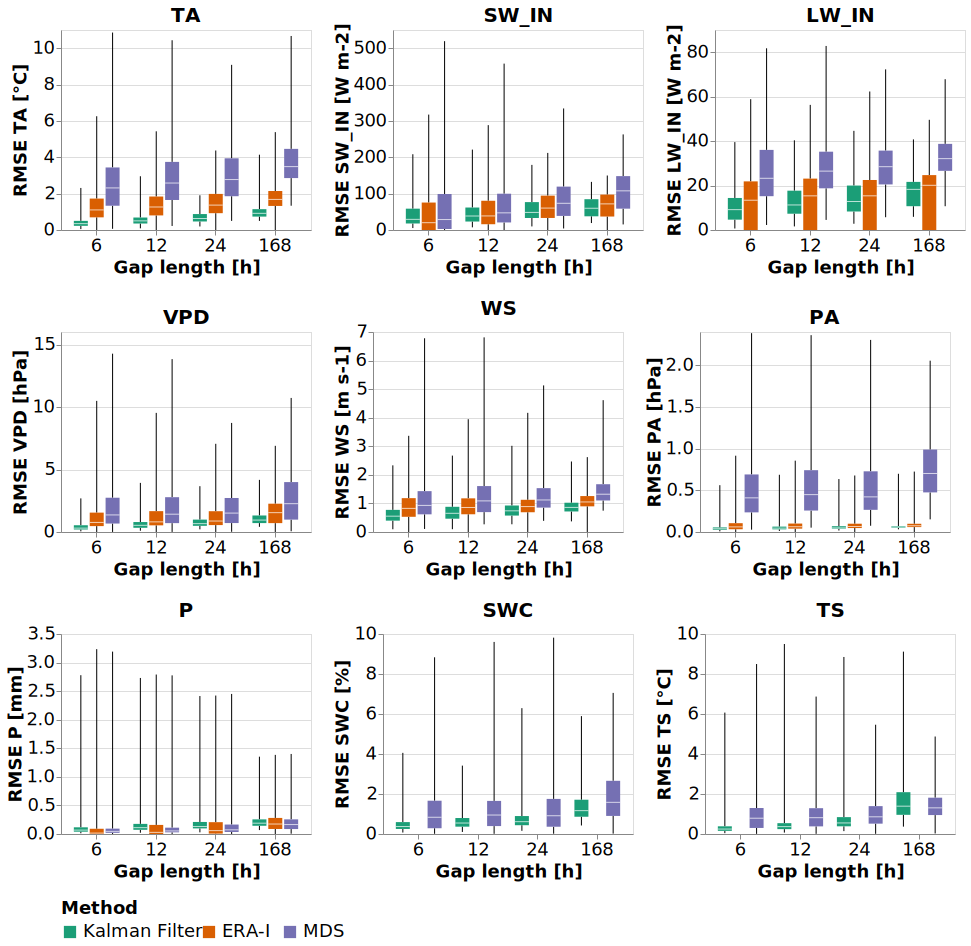
\includegraphics[width=\imgwidth]{images2/the_plot}}
\caption{ Imputation performance of the Kalman filter in comparison to the state of art methods: ERA-Interim (ERA-I) and Marginal Distribution Sampling (MDS) to compare. The performance was assessed calculating for each method the \textit{Root Mean Square Error} (RMSE) for an artificial gap, with a single variable missing. For each combination of variable and gap length a sample of 500 random gaps has been used (total 18000 artificial gaps).
The Kalman Filter model has been fine-tuned to each variable. ERA-I dataset doesn't contain \texttt{TS} and \texttt{SWC} so cannot be used for their imputation. The extent of the box plot vertical lines represent the maximum and minimum value.}
\label{fig:the_plot}
\end{figure}

\begin{table}
\centering
\caption{\CapTheTable}
\label{tbl:the_table}
\begin{tabular}{p{2.1cm}l|rr|rr|rr}
\toprule
 &  & \multicolumn{2}{r}{Kalman Filter} & \multicolumn{2}{r}{ERA-I} & \multicolumn{2}{r}{MDS} \\
 & RMSE & mean & std & mean & std & mean & std \\
Variable & Gap &  &  &  &  &  &  \\
\midrule
\multirow[c]{4}{*}{\parbox{2.1cm}{\textbf{TA} [\si{°C}]}} & 6 h & \bfseries 0.405 & 0.258 & 1.347 & 0.998 & 2.713 & 1.897 \\
 & 12 h & \bfseries 0.607 & 0.401 & 1.472 & 0.901 & 2.942 & 1.748 \\
 & 1 day (24 h) & \bfseries 0.741 & 0.368 & 1.530 & 0.800 & 3.013 & 1.611 \\
 & 1 week (168 h) & \bfseries 1.021 & 0.445 & 1.754 & 0.643 & 3.780 & 1.315 \\
\cline{1-8}
\multirow[c]{4}{*}{\parbox{2.1cm}{\textbf{SW\_IN} [\si{W/m^2}]}} & 6 h & \bfseries 44.637 & 40.465 & 49.333 & 66.242 & 63.537 & 85.402 \\
 & 12 h & \bfseries 48.155 & 33.868 & 54.208 & 49.769 & 69.427 & 68.936 \\
 & 1 day (24 h) & \bfseries 56.564 & 30.043 & 65.950 & 40.931 & 86.771 & 59.604 \\
 & 1 week (168 h) & \bfseries 61.583 & 25.740 & 70.224 & 34.883 & 107.384 & 53.606 \\
\cline{1-8}
\multirow[c]{4}{*}{\parbox{2.1cm}{\textbf{LW\_IN} [\si{W/m^2}]}} & 6 h & \bfseries 10.902 & 7.736 & 13.805 & 12.988 & 26.680 & 15.022 \\
 & 12 h & \bfseries 13.422 & 7.735 & 14.767 & 12.585 & 28.085 & 13.457 \\
 & 1 day (24 h) & 14.594 & 7.840 & \bfseries 14.093 & 12.228 & 29.614 & 12.417 \\
 & 1 week (168 h) & 17.063 & 6.425 & \bfseries 16.366 & 11.130 & 32.955 & 8.834 \\
\cline{1-8}
\multirow[c]{4}{*}{\parbox{2.1cm}{\textbf{VPD} [\si{hPa}]}} & 6 h & \bfseries 0.428 & 0.363 & 1.297 & 1.547 & 2.084 & 2.149 \\
 & 12 h & \bfseries 0.661 & 0.505 & 1.265 & 1.289 & 2.137 & 2.096 \\
 & 1 day (24 h) & \bfseries 0.828 & 0.502 & 1.248 & 1.032 & 1.912 & 1.605 \\
 & 1 week (168 h) & \bfseries 1.126 & 0.633 & 1.662 & 1.127 & 2.661 & 1.965 \\
\cline{1-8}
\multirow[c]{4}{*}{\parbox{2.1cm}{\textbf{WS} [\si{m/s}]}} & 6 h & \bfseries 0.617 & 0.317 & 0.912 & 0.508 & 1.136 & 0.783 \\
 & 12 h & \bfseries 0.715 & 0.351 & 0.957 & 0.524 & 1.261 & 0.797 \\
 & 1 day (24 h) & \bfseries 0.802 & 0.343 & 0.949 & 0.447 & 1.276 & 0.609 \\
 & 1 week (168 h) & \bfseries 0.950 & 0.363 & 1.089 & 0.349 & 1.495 & 0.615 \\
\cline{1-8}
\multirow[c]{4}{*}{\parbox{2.1cm}{\textbf{PA} [\si{hPa}]}} & 6 h & \bfseries 0.045 & 0.034 & 0.075 & 0.062 & 0.531 & 0.441 \\
 & 12 h & \bfseries 0.053 & 0.042 & 0.077 & 0.058 & 0.564 & 0.427 \\
 & 1 day (24 h) & \bfseries 0.059 & 0.039 & 0.079 & 0.051 & 0.557 & 0.404 \\
 & 1 week (168 h) & \bfseries 0.066 & 0.048 & 0.084 & 0.054 & 0.773 & 0.384 \\
\cline{1-8}
\multirow[c]{4}{*}{\parbox{2.1cm}{\textbf{P} [\si{mm}]}} & 6 h & 0.134 & 0.274 & \bfseries 0.113 & 0.316 & 0.118 & 0.306 \\
 & 12 h & 0.179 & 0.295 & 0.139 & 0.297 & \bfseries 0.130 & 0.281 \\
 & 1 day (24 h) & 0.206 & 0.254 & 0.166 & 0.288 & \bfseries 0.159 & 0.265 \\
 & 1 week (168 h) & 0.240 & 0.174 & 0.223 & 0.202 & \bfseries 0.215 & 0.197 \\
\cline{1-8}
\multirow[c]{4}{*}{\parbox{2.1cm}{\textbf{SWC} [\si{\%}]}} & 6 h & \bfseries 0.508 & 0.487 & - & - & 1.314 & 1.557 \\
 & 12 h & \bfseries 0.665 & 0.472 & - & - & 1.278 & 1.323 \\
 & 1 day (24 h) & \bfseries 0.779 & 0.641 & - & - & 1.356 & 1.472 \\
 & 1 week (168 h) & \bfseries 1.494 & 0.948 & - & - & 1.948 & 1.488 \\
\cline{1-8}
\multirow[c]{4}{*}{\parbox{2.1cm}{\textbf{TS} [\si{°C}]}} & 6 h & \bfseries 0.341 & 0.432 & - & - & 0.954 & 0.889 \\
 & 12 h & \bfseries 0.534 & 0.784 & - & - & 1.003 & 0.877 \\
 & 1 day (24 h) & \bfseries 0.787 & 0.852 & - & - & 1.078 & 0.857 \\
 & 1 week (168 h) & 1.660 & 1.078 & - & - & \bfseries 1.440 & 0.764 \\
\cline{1-8}
\bottomrule
\end{tabular}
\end{table}


The performance of the KF for each variable is analysed in detail and compared with the other methods

\paragraph{Air Temperature} Air temperature is the variable with the biggest improvement in performance, up to XX for 6 hours long gaps. KF outperforms ERA-I also for long gaps and the compared to MDS there is a 77\% reduction in the RMSE. The visual inspection of the time series indicate an overall very good reconstruction on the missing data. 

\paragraph{Incoming shortwave radiation} The KF is the method with the smaller average RMSE, but the relative improvement is small, only 12\% compared to ERA-I. The highest error is at night, where \vv{SW\_IN} is by definition always 0, but the KF often predicts sudden changes with errors in the order of 50 \si{W/m^2}. However, this means that during the day the KF is consistently better than other methods, which is also confirmed by visual inspections of the time series. The main factor behind the changes in \vv{SW\_IN} is the cloud cover, which ERA-I often correctly predicts and consequently the KF can access this information, while the MDS is unable to model this type of changes.

\paragraph{Incoming Longwave radiation} The imputation performance of the KF is comparable with ERA-I. For short gaps KF is better (20 \% improvement for 6 hours long gaps). This can be visualized in figure \ref{fig:ts_2_0}, where in the 12 hours long gap ERA is incorrect by an offset of roughly 50 \si{W/m^2}, while the KF prediction is more accurate towards the edges of the gap. KF The imputation performance of MDS is poor, especially for long gaps.

\paragraph{Vapour Pressure Deficit} KF is the best model for all gap lengths, the relative performance is higher for short gaps (XX compared to ERA) and progressively smaller for longer gaps. The analysis of the time series suggest that the KF is overall good at reconstructing the higher frequency changes of \vv{VPD}, but in some scenarios KF wrongly predicts short term variation (gap 1 week figure \ref{fig:ts_2-1}).

\paragraph{Wind Speed} The KF is the best method imputation method for all gap lengths, with an average error reduction of 21\% compared to ERA-I. The wind speed is the variable with the highest standardized RMSE (appendix figure \ref{fig:the_plot_stand}), which indicates that the RMSE is high compared to the \vv{WS} standard deviation. The visual inspection of the time series (figure \ref{fig:ts_2-1} and \ref{fig:ts_3-1}), indicates that the \vv{WS} has a high variability on a short time scales, which is not captured by ERA-I nor by the KF.

\paragraph{Air Pressure} The imputation error of \vv{PA} is low for KF and ERA-I. The KF outperforms ERA-I with an improvement ranging from 36\% for 6 hours gaps to 20\% for 1 week long gaps. The visual analysis of the time series suggest that the KF slightly overestimate the short term variability for \vv{PA}. MDS is significantly worse, with the imputation error an order of magnitude bigger than ERA-I.

\paragraph{Precipitation} The Precipitation is a variable where no methods perform well, with models in some case predicting precipitation event that do not exist and in other missing the real precipitation. The RMSE of the three methods is comparable. However, the RMSE is not a suitable metric for \vv{P}, due to the very high number of data points with no precipitation. For reference, the RMSE of a null model (i.e. always predicts 0) is 0.28 \si{mm}, which is comparable with the errors of all imputation methods. 
The visual analysis of the time series shows that ERA-I predictions are the one that are physically realistic, even though the precipitation amount is often incorrect, while the KF often predicts negative values for \vv{P}, which is physically impossible and MDS in a tested scenario (Appendix figure \ref{fig:ts_2-2}) predicts an highly unlikely constant low amount of \vv{P}.

\paragraph{Soil Water Content} The KF is the best imputation method, for short gaps there is an error reduction of 61\% compared to MDS, while for long gap (1 week) the absolute error of the KF roughly doubles and the improvement is performance is limited to 23\%. \vv{SWC} is a variable that is not available in ERA-I, so KF and MDS are the only available methods. Moreover, the KF does not have a control variable for \vv{SWC}.
The analysis of the time series shows that the mean of KF prediction is overall accurate, and notably manages also to predict sudden changes in \vv{SWC} (figure \ref{fig:ts_1-2}). However, the KF constantly predict small variations in the soil water content, which are not reflected in the observations.

\paragraph{Soil Temperature} The KF is the best imputation method for short gaps (less than 24 hours), but the MDS is better for 1 week long gaps (Figure \ref{fig:the_plot}). For short gaps there is an big difference in the methods error (up to 60\%), but is reduced for long gaps (KF is 15\% worse than MDS). In two of the long time series analysed the \vv{TS} is almost constant (figure \ref{fig:ts_1-2} and \ref{fig:ts_3-2}), but the KF incorrectly predicts important variations, while the MDS is overall constant. In another scenario (appendix figure \ref{fig:ts_2-2}), where there is a diurnal pattern in \vv{TS}, the KF predictions have an overall correction shape, even though there is roughly 1 \si{°C} error.

% \begin{itemize}
%     \item \vv{TA}: KF good performance and improvement over ERA. For long gaps follows ERA but often better. For reference, the accuracy of the thermometer installed at Hainich \cite{noauthor_associated_2020} is 0.1 \si{°C} \cite{noauthor_specification_nodate}.
%     \item \vv{SW\_IN}: KF performance at night is not good, there are negative values up to -50 and then a lot of variation even though should be constant at 0 and the control variable is correct. During the day methods are comparable with often Kalman Filter having the best performance 
%     \item \vv{LW\_IN} KF compare performance ERA. ERA has a much wider range of errors, for some gaps is very good for others is quite worse. MDS is quite bad basically predicting a constant value and the come drastic changes. LW\_IN has a "blocky" behaviour that is correctly predicted by ERA
%     \item \vv{VPD}. KF is better especially for short gaps. MDS not very good miss variation at night (probably due to no change in SW\_IN)
%     \item WS has the worse standarized RMSE, a lot of short term variability that no model captures. KF still best results 
%     \item \vv{PA} KF consistently better then ERA. For MDS error 1 order of magnitude bigger
%     \item P KF worse performance than other methods, but still similar performance
%     \item SWC KF has on average a better performance than MDS, especially for short gaps. However, the time series of KF are not very good. The variation in the predicted time series is often much higher than the actual one (Figure \ref{fig:ts_2_0} \ref{fig:ts_2_1} \ref{fig:ts_2_2}). ERA is not available
%     \item TS KF has on average a better performance than MDS, especially for short gaps. However, the time series of KF are not very good. The variation in the predicted time series is often much higher than the actual one when there is a small variation in the variable(Figure \ref{fig:ts_2_0} gap length 6h and 12h) conversely is much better when there is variation (Figure \ref{fig:ts_2_1} \ref{fig:ts_2_2}). the KF models correctly the increase and decrease in soil temperature even though if the values may not be accurate. ERA is not available
    
% \end{itemize}




% \subsubsection{Example Time series}

\newgeometry{top=.1in}
\begin{figure}
\centerline{\includegraphics[width=\imgwidth]{images2/timeseries_1}}
\caption{Illustration of the imputation \texttt{TA}, \vv{SW\_IN}, \vv{LW\_IN}, \vv{VPD}, \vv{WS} using different methods: Kalman Filter, ERA-Interim (ERA-I) and Marginal Distribution Sampling (MDS). The methods are compared by visualizing the time series of an artificial random gap for a three gap lengths. . For each variable, 3 random artificial gap (length 6 hours, 12 hours, 1 week) are imputed using the three methods: Kalman Filter (green), ERA-I (orange), MDS (purple).  For the Kalman Filter the shared area show the uncertainty of the prediction $+/- 2 \sigma$. The grey shaded area and the vertical black lines delimit the artificial gaps, where the observations are not available to the model but are used to assess the imputation performance. The ERA-I prediction is the control variable of the Kalman Filter.}
\label{fig:ts_1-1}
\end{figure}
\restoregeometry

\begin{figure}
\centerline{\includegraphics[width=\imgwidth]{images2/timeseries_2}}
\caption{Illustration of the imputation \texttt{PA}, \vv{P}, \vv{SWC}, \vv{TS} using different methods: Kalman Filter, ERA-Interim (ERA-I) and Marginal Distribution Sampling (MDS). The methods are compared by visualizing the time series of an artificial random gap for a three gap lengths. . For each variable, 3 random artificial gap (length 6 hours, 12 hours, 1 week) are imputed using the three methods: Kalman Filter (green), ERA-I (orange), MDS (purple).  For the Kalman Filter the shared area show the uncertainty of the prediction $+/- 2 \sigma$. The grey shaded area and the vertical black lines delimit the artificial gaps, where the observations are not available to the model but are used to assess the imputation performance. The ERA-I prediction is the control variable of the Kalman Filter.}
\label{fig:ts_1-2}
\end{figure}

% \textbf{goal} Show how a Kalman Filter Gap filling looks like and the uncertainty 

% \begin{figure}
% \centerline{\includegraphics[width=6in]{timeseries_1}}
% \caption{Timeseries 1}
% \end{figure}

% \begin{itemize}
%     \item a few sample variables (max 3/4)
%     \item a representative gap length
%     \item manually choose interesting gaps (2-4)
%     \item no gap in other variable
% \end{itemize}

% This is the most intuitive way of looking at gap filling and can select the gaps for highlighting the strengths and weakness of the filter


\subsection{Aspect affect Kalman Filter performance}

\subsubsection{Gap Length}

The effect of the gap length on the KF imputation performance is analysed by measuring the RMSE on gaps in a single variable for lengths ranging from 1 hour to 1 week (figure \ref{fig:gap_len} and appendix table \ref{gap_len}). For the majority of the variables the error increases with the gap length only up to 24 hours and then is overall constant. For three variables (\vv{P}, \vv{SWC} and \vv{TS}) the imputation error keep increasing after 24 hours, but the rate decreases with the gap length. In all cases, the biggest change in the error happens between 1 hours and 12 hours long gaps.

For all variables, there is a significant difference in the error of very short gaps (1 hour) and long gaps (1 week) in all variables, on average the error for gaps 1 hour long is the 31\% of the one for 1 week long gaps.
The variability in the RMSE between gaps (i.e. std in appendix table \ref{gap_len}) is roughly constant between the different gap lengths.

% \begin{itemize}
%     \item short gaps have a smaller error
%     \item then there is a steep increase for gaps up to 24 hours
%     \item after 24 hours the is no or little change into the error
%     \item the variability on of the error between gaps (std of RMSE) follows a similar partner
%     \item \vv{P} and \vv{SWC} and \vv{TS} are an exception from this pattern, with both the mean and std oft the error increasing for gaps longer than a day
% \end{itemize}



% \textbf{goal} impact of the gap length on the gap filling
\begin{figure}
\centerline{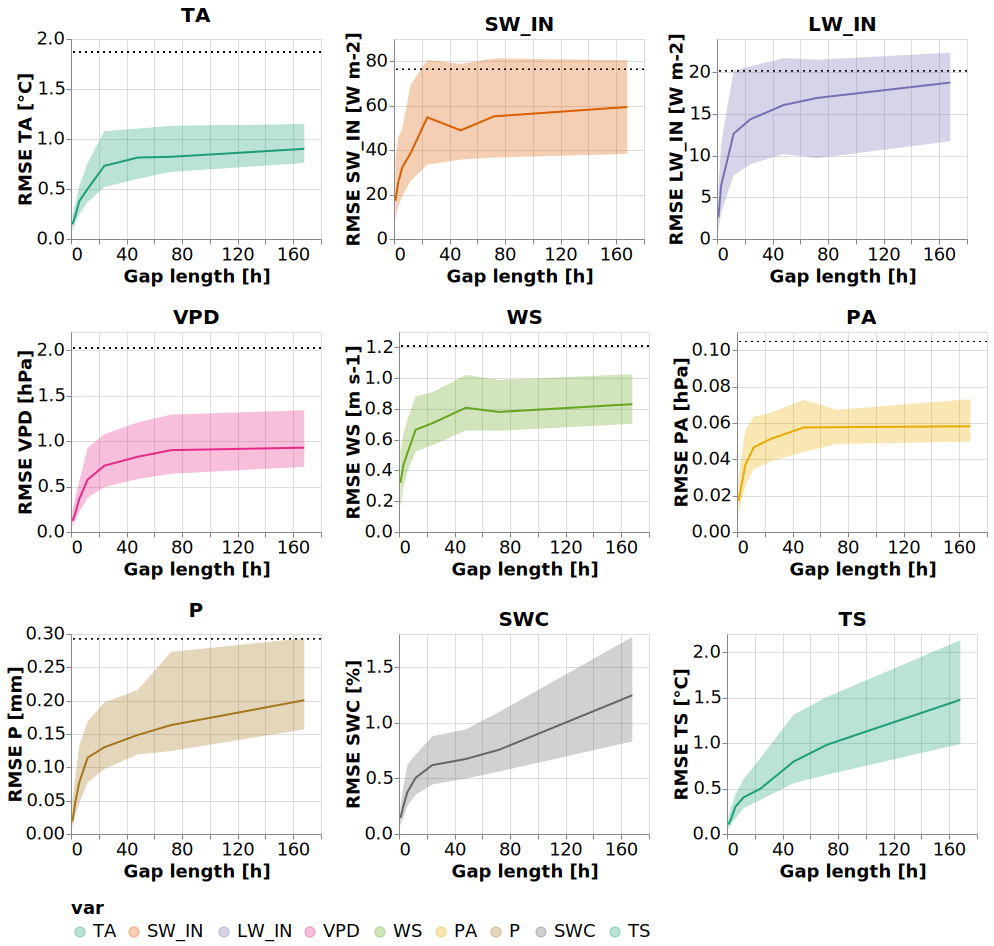
\includegraphics[width=\imgwidth]{images2/gap_len}}
\caption{Effect of gap length on the KF performance. The solid line shows the median RMSE, while the shaded area is delimited by the first and third quartile. The dotted black line is the mean ERA-I error for the entire dataset (ERA-I data is not available for \vv{SWC} and \vv{TS}). Seven different gaps lengths were tested (1 hour, 3 hours, 6 hours, 12 hours, 1 day, 2 days, 3 days, 1 week), for each of them 500 artificial gaps were generated for each variable (total 31500 gaps). For each variable, the fine-tuned KF model has been used (\textit{KF-\textlangle var\textrangle-Sin-6\_336} figure \ref{fig:training})}
\label{fig:gap_len}
\end{figure}


\subsubsection{Control variables}

The importance of the control variables is assessed by comparing the imputation error of a model that uses the control variables (\textit{KF-Gen-Sin-6\_336}) with a model that does not have access to the control variables (\textit{KF-Gen-Sin-6\_336-No\_Contr}). Both models are not fine-tuned for each variable, but are generic.
In general, the control variables improve the importation performance for all variables for all gap lengths. The exceptions are \vv{P} and \vv{TS}, where the use of the two models are equivalent, and for short gaps (6 hours) in \vv{SWC} and \vv{WS}.
For all variables, the longer the gap, the biggest the performance improvement of the model with the control variables (Appendix table \ref{control}). Notably, the use of the control variables improve the prediction performance for \vv{SWC}, even though is a variable that is not present in ERA-I.
The variable where the use of the control results in the biggest improvement is \vv{PA}, where for gaps 1 week long the model without the control has an error almost 6 times bigger than the one with the control.

% \begin{itemize}
%     \item generic model with control vs generic model without control
%     \item for short gaps the use of the control is increasing the error
%     \item for longer gaps the control is usually helping
%     \item for \vv{SWC} and \vv{TA} using the control is slightly worse
%     \item for \vv{PA} the error without control is much higher around 5 times bigger for 1 week long gaps.
%     \item for \vv{P} control is helping a bit
% \end{itemize}

% \textbf{goal} show how the use of the control (ERA-5 data) in the gap is impacting the predictions

% \includegraphics[width=\textwidth]{use_control}

\begin{figure}
\centerline{\includegraphics[width=\imgwidth]{images2/use_control.png}}
\caption{Comparison between KF with control variables (in green \textit{KF-Gen-Sin-6\_336}) and KF without control variable (in purple \textit{KF-Gen-Sin-6\_336-No\_Contr}). For each combination of variable and each gap length, 500 artificial gaps were created.}
\label{fig:control}
\end{figure}

\subsubsection{Gaps in multiple variables}

The importance of the inter-variable correlation for the KF predictions has been assessed by comparing the imputation for a gap with only one variable missing and then same gap with all variables missing. All the gaps were imputed using the same model, \textit{KF-Gen-Multi-6\_30} (Figure \ref{fig:training}) and the gap length is limited to 15 hours due to numerical stability issues.

The presence of other variables in the gap is overall improving the model predictions, for some variables there is a significant error reduction (e.g. around 40 \% for \vv{TA}) but for others the improvement is minimal (e.g. less than 2\% for \vv{WS}). The pattern  pattern described by the inter-variable correlation, the improvement is minimal for variable that have a low correlation with others 

Across the different variables, there is an increase in the absolute values of the difference in RMSE with an increase in gap length.
% \begin{itemize}
%     % \item the max gap length is 15 because after that the model crashed due to numerical stability issues
%     \item compare a specialized model with gap in only one var and a generic model trained with gaps in all variables
%     \item Overall for short gaps variable correlation doesn't help much and actually is worse
%     \item for \vv{TA} presence other variables helps to reduce error and variability of error
%     \item for \vv{SW\_IN} worse with other variables for gap of 15 hours
%     \item for \vv{VPD} and \vv{WS} other variable help reducing both mean and std for RMSE 
%     \item for \vv{P} other variables increase error
%     \item \vv{SWC} the RMSE is higher when there are other variables in the gap
%     \item for \vv{TS} when there are other var err higher for short gaps but then comparable
% \end{itemize}

\begin{figure}
\centerline{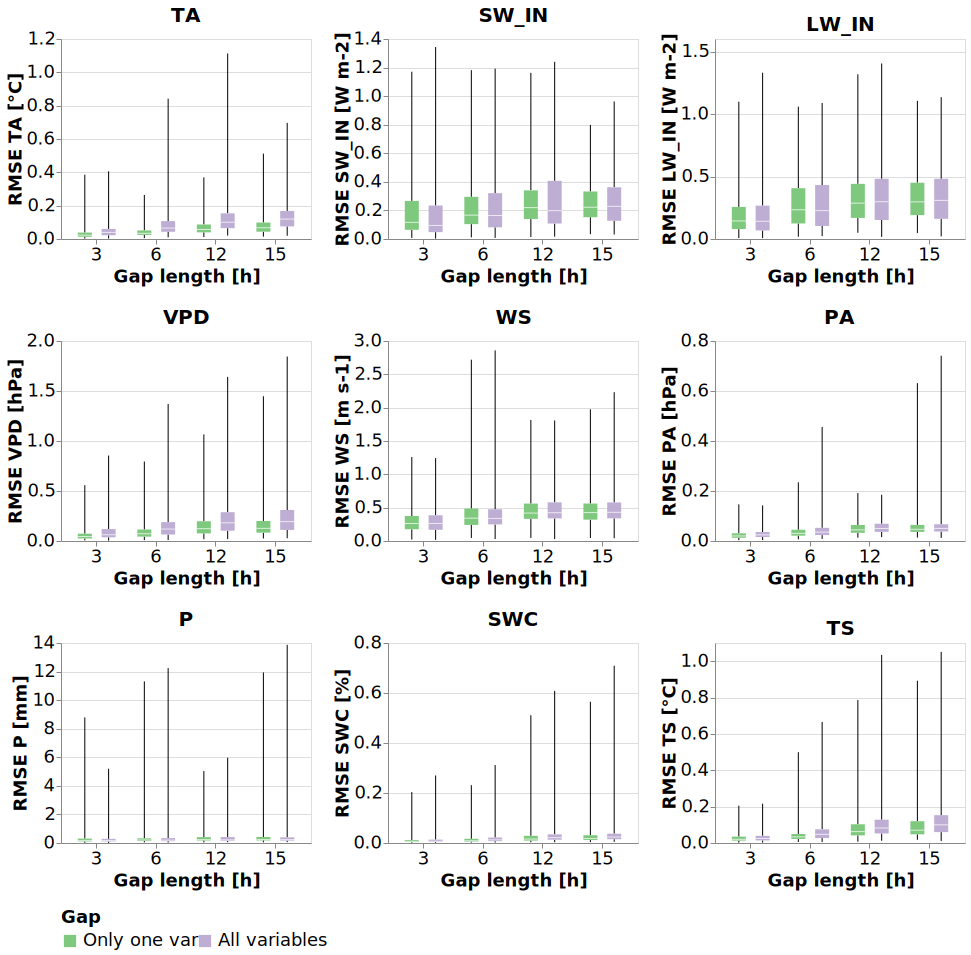
\includegraphics[width=\imgwidth]{images2/gap_single_var}}
\caption{Gap single var}
\label{fig:gap_single_var}
\end{figure}

\subsection{Kalman Filter training}

\subsubsection{Variable fine-tuning}

The performance of the KF is improved if the model is fine-tuned with gaps only for one variable (e.g. only for \vv{TA}). For each variable a different model has been used (\textit{KF-\textlangle var \textrangle-Sin-6\_336}) and the performance compared to a generic model that has been trained with one gap in any variable (\textit{KF-Gen-Sin-6\_336}). For each combination of gap length and variable, 500 artificial gaps were created.

The fine-tuning is reducing the error for all the variables (figure \ref{fig:generic} and appendix table \ref{ta} \ref{fig:generic})
\begin{itemize}
    \item fine-tuning the model is improving the performance across all variables
    \item biggest increase is in \vv{SWC} and \vv{TA}, which much smaller error especially for long gap. Variability of RMSE also decreases
\end{itemize}

\begin{figure}
\centerline{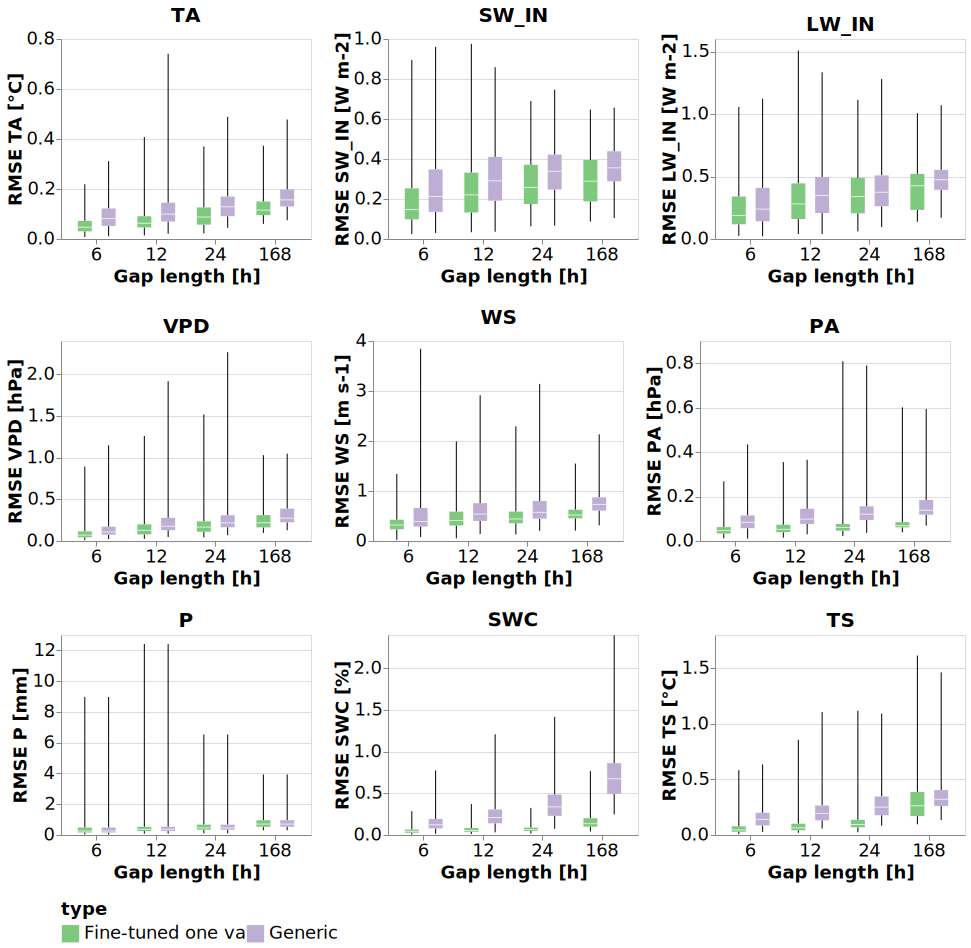
\includegraphics[width=\imgwidth]{images2/generic.png}}
\caption{Comparison model fine-tuned for each variable (green) with generic model (purple). 100 samples for each variable and gap length}
\label{fig:generic}
\end{figure}

\subsubsection{Training limitations}

\begin{figure}
\centerline{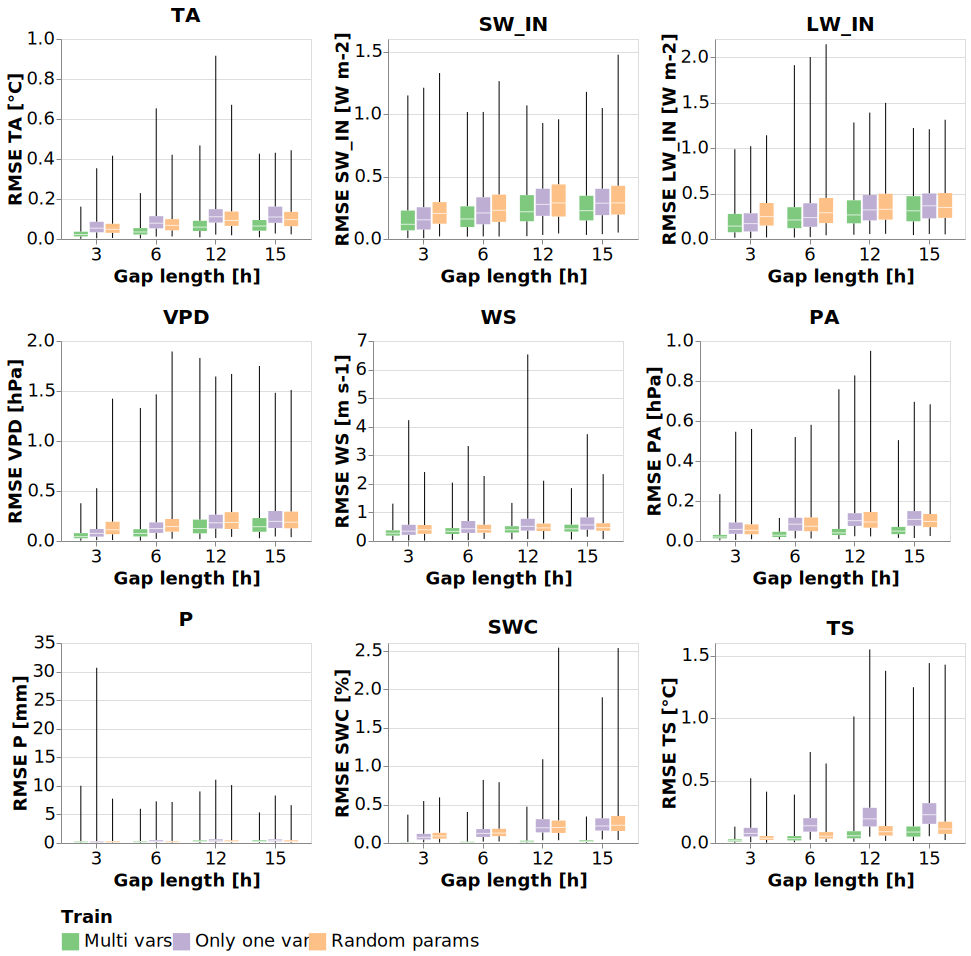
\includegraphics[width=\imgwidth]{images2/train_compare.png}}
\caption{Comparison of different training conditions}
\label{fig:train_compare}
\end{figure}


\section{Discussion}




\subsection{Kalman Filter performance}

The results confirm the hypothesis that temporal autocorrelation is a key approach for imputing gaps in meteorological variables. One of the biggest strength of the KF is that it make better use of temporal autocorrelation, which is the likely the biggest single factor behind the improved performance. The fact that the error is increasing with the gap length only for the first 24 hours is confirming this. Moreover, the variables the relative performance of the filter is higher for variables that have a higher temporal correlation (\vv{TA}, \vv{PA} and \vv{VPD})

The improvement of KF performance across all variables when including the control variables confirms the hypothesis that the combination of the imputation approaches can produce better predictions. In line with the expectations, the use of the ERA-I data is crucial for the filter performance for long gaps, but results only in limited improvements for short gaps. Notably, the use of the control improve the predictions also for \vv{SWC} and \vv{TS}, which even if they are directly present in the ERA-I dataset, they correlated with other variables that are present in the control.

The results suggest that depending on the length of the gap the optimal imputation strategy is different, for short gaps the most important aspect is the temporal autocorrelation, while for longer gaps the control variable and inter-variable correlation plays a bigger role. This is expected, as for many variable the observations before and after the gap can provide a lot of information to reconstruct the missing data, but the effect is reduced with the gap length and other source of information are needed to correctly model the missing variable.

The numerical stability issues limited our analysis of the effect of the inter-variable correlation for short gaps, where we expect the effect to be limited. In fact, the presence of the information of other variables
The results, for the of figure \ref{fig:gap_single_var}, highlight a limitation of the model training. The model trained with the gap in  only one variable, should be able to learn to ignore the information of the other variable and achieve the same performance as the model trained with gaps in all variables. However, this is not the case, which is likely due to the optimizer finding a local minimum.
The low importance of inter-variable correlation may also depend on the parameter initialization, where each observed variables is directly mapped to a state variable. This issue in the model training may be the source of the excessive variability in the predictions of  \vv{TS} and \vv{SWC}.
Further research would be needed to understand the behaviour of the model training and the impact of the initial parameters.

The best imputation of the KF is achieved only when the model parameters are fine-tuned to the specific conditions. We tested the fine-tuning of the model both to one variable and to short gaps, with both scenarios producing an increase in the performance. Moreover, we expect that further tuning the model to more granular conditions would improve the performance. For instance, the rate of change of the soil temperature is significantly  higher in dry summer day compared to winter day with the ground covered in snow. Therefore, the optimal KF parameters would be different between those conditions.

\paragraph{Variables considerations}

\subparagraph{Shortwave radiation} The low performance of the \vv{SW\_IN} at night highlights a limitation of the Kalman filter.  At its core the filter considers only the evolution of the filter between consecutive time steps, and since  hence it cannot model the daily pattern of \vv{SW\_IN}. Moreover, the rate of change of \vv{SW\_IN} between consecutive time steps is between the day and the night is very different and since the KF uses constant parameters cannot include this variability. The control variable is the main source of information for the filter, which is confirmed by the results.

\subparagraph{Precipitation} The precipitation has a low temporal autocorrelation and low correlation with other variables, this significantly limits the ability of the KF to accurately impute missing values. The accuracy of ERA-I is limited as well, in  bias correction is done using annual sums and not the precipitation at 30 mins intervals, because the timing is considered not accurate enough. Moreover, there is no precipitation in the majority of the observations (over 90\% data points in Hainich), for which the RMSE is a well suited metric. In fact, \cite{chivers_imputation_2020} developed a spatial and temporal imputation method for precipitation, that employs two different models: first they predict for each data point, whether there is precipitation or not and then use another models to predict the amount of precipitation.  Overall the precipitation has a high spatial and temporal variability \cite{mital_sequential_2020} and different characteristics  than other meteorological variable. The KF is not suited for the imputation precipitation, which would require a tailored modelling approach that is beyond the scope of this work.

\subparagraph{Wind Speed} The KF doesn't model accurately the high frequency variation of the wind speed, and is the variable with the highest standardized RMSE. This is consistent with the results \cite{vuichard_filling_2015}. The KF cannot extract the information about the high frequency variation from other observations of the wind sped, but KF is able to model higher frequency variations only if the information is present in either the control variable or in other variables. For the case of the wind speed this is not the case, as ERA-I has this limitation and no other variable has a high correlation with the wind speed. This limitation of ERA-I is also the likely reason behind the increased error in \vv{WS} when using the control for short gap length, where low variability in ERA-I is negatively affecting the model prediction.
This is scenario shows the limitations of the simplicity KF, while a properly designed Gaussian Process should be able to model the high frequency variation. Nonetheless, the KF has a better performance than the current imputation methods. 


\paragraph{Training}

\paragraph{Numerical stability} becomes not positive definite, hence is impossible to compute the log likelihood
appendix figures

\subsection{Kalman Filter application}

\paragraph{} Our results suggest that a Kalman Filter can be employed to improve the imputation of meteorological variables for EC applications, especially for gaps shorter than one day. 
The highest error reduction is for short gaps (less than 1 day) and  in particular for the air temperature. We expect that is relevant to reduce error in Land Surface Models, as they work on short time scales and the temperature is a key driver of core ecosystem processes. Processed like photosynthesis or respiration have a strong non-linear dependency on temperature, making inaccuracies on the temperature relevant for  \cite{bonan_climate_2019-2}.
The relative performance of KF is reduced for medium gaps (1 week) and we assume that for longer gaps the error of the KF is going to get progressively closer to the ERA-I one. Nonetheless, the KF can be successfully applied to impute long gaps for variable that are not available in ERA-I (e.g. \vv{TS} or \vv{SWC}) as it exploits the ERA-I observations for other variables and the inter-variable correlation.

In any scenario, the KF provides an interpretable estimate of uncertainty. Currently, I am not aware of any imputation methods that provide an interpretable uncertainty and thus no application have been developed for it. However, the ability to accurately assess the quality of the gap filling for each data point can be important to an effective use of the imputed time series.

\paragraph{} The current KF implementation has two limitations that would prevent the application in a production scenario: numerical instability when all variables are missing for more than 15 hours, physically impossible predictions of \vv{SW\_IN} at night. However, I believe that the first two limitations are relatively straightforward to overcome, as suggested in the following section. The deployment of the KF may be impacted by the need to fine-tune the model parameters to achieve the best performance. This is inherited to the KF structure.
The current models is using 9 different KF, each of them optimized for one variable. This means that while it is possible to run the KF to impute gaps all variables, the best results are only achieved when imputing each variable separately. Moreover, I tested the KF only one site, but from the results of \cite{vuichard_filling_2015} show that the accuracy of ERA-I, so the control variable parameters would likely need to fine-tuned to each variable. In addition, in the current implementation fine-tuning procedure requires a manual intervention to interrupt the training process and avoid overfitting the model.
The necessity to fine-tune the KF to a specific conditions is a not critical limitation, but it is necessary to consider the increased computation cost and the deployment complexity. 


\subsection{Future Outlook}

\paragraph{Model improvements} This work builds the foundations to have a KF based method for imputing meteorological variables. However, we believe that there are at least two that are required before considering using the model in production.

The numerical instability of the current KF implementation limits the gaps to 15 hours when all variables are missing. The current implementation is a hybrid between a square root filter and standard Kalman Filter. The use of the full covariance matrices in the smoothing pass and the in the log-likelihood computations is the source of the numerical instability. More research is needed on developing a suitable formulation of a square root smoother, which the available literature suggest that is possible to derive \cite{rutten_square-root_2013, park_new_1996}. 

The KF often predicts negatives values of the shortwave radiation at night, that are physically impossible. However, imputing shortwave radiation at night is a simple problem since is always zero and the exact time of the sunrise and sunset can be computed from the day of the year and the geographic coordinates. Therefore the KF can be used to impute only the values during the day, where it is the method with the best performance.

I identify further directions...

\subparagraph{ERA-5 Land} The European Centre for Medium-Range Weather Forecasts recently released two new weather reanalysis datasets: ERA5 in 2020 \cite{hersbach_era5_2020} and ERA-5 Land  in 2021 \cite{munoz-sabater_era5-land_2021}, which supersede the ERA-Interim dataset. The ERA5-Land dataset coves only the continent, but has a much higher spatial resolution (9 km vs 80km) ad higher temporal resolution (1 hour instead of 3 hour). The use ERA5-Land data as control variable for the KF has the potential to improve the imputation performance.

\subparagraph{Parameter initialization and Training} Our analysis suggest initial parameters have significant influence on the final parameters and thus the performance of the model. There are several approaches to initialize a Kalman Filter \cite{durbin_time_2012-4} and a robust comparison between the different methods may reveal a better initialization strategy than the linear trend model.  

\subparagraph{Model Filter Parameters} One of the advantages of the iterative nature of the KF formulation is the ability to change the parameters between time step. This opens the possibility to have a model that predicts the parameters of the filter depending on the conditions, which should overcome the necessity to fine-tune the KF parameters to each condition. 

\subparagraph{Non-linear transformation control} The KF now has a linear , but the real relationship is not linear . The formulation of the Kalman Filter doesn't constraint the control variable transformation to be linear, thus a model the ERA data can be processed with a more powerful model, which as a Neural Network. The implementation of the KF using PyTorch simplify such additions.

\subparagraph{Observations noise} The uncertainty of the observations can be estimated from the instrument accuracy and used as input of the model to avoid underestimating the uncertainty of the observations. For instance, the typical accuracy of a shortwave measurement is in the order of 10 \si{W\m^2}, which is comparable to the uncertainties of the model.

\paragraph{Model Evaluation} This study provides a first evaluation of the imputation performance of different, but a more in-depth analysis contribute to understand the impact in the real impact of the imputation methods.

The first aspect is to test the imputation performance usgin observations from different sites

Another aspect to consider is that the meteorological data is not missing completely at random. Further research would be needed, but is reasonable to assume that there is a correlation between the gaps of different variable and that the time of the year has an impact on data availability. One reason that can contribute to patterns in the missing that is the fact that the air temperature and vapour pressure deficit are often measured from the same sensor (eg. \cite{noauthor_specification_nodate}), which increase the likelihood of both variable missing at the same time. Another scenario is a station that uses solar panels, which are more likely to have power failure during winter. A robust assessment of the imputation performance should include missing data with realistic patterns.

The metric used for the evaluation is also important. The RMSE is limited to time series measure the average distance between the predictions and the observations, but doesn't compare characteristics of the time series such as the variance, the shape of the presence of a time-shift \cite{guen_shape_nodate}. The use of additional metrics (eg. DILATE \cite{guen_shape_nodate}) can improve the understanding of the quality of the imputation.

Finally, the impact of the KF imputation can be evaluated by the reduction in the error of Land Surface Models compared to state of the art methods. Improving the quality of the predictions of Land Surface Models is arguably the main reason to use KF imputation. This can be assess directly by running a Land Surface Model with a complete time series, and the one of application of imputed meteorological ....


\section{Conclusions}

\begin{itemize}
    \item Kalman Filter from preliminary results have the potential to improve imputation of meteo data
    \item on all tested variables smaller or comparable error than other methods, but P
    \item lower variability
    \item provide interpretable uncertainty
    \item limitations implementation
    \begin{itemize}
        \item numerical stability
        \item SW\_IN
    \end{itemize}
    \item need to fine tune parameters is a limitation of the model
    \item can test different init parameters and effect of model training
    \item potential for further development
    \item robust assessment of performance in real life conditions and test different sites
\end{itemize}


\printbibliography

\appendix

\FloatBarrier


\section{Additional Results}

\subsection{Comparison to other imputation methods}

\begin{figure}
    \centerline{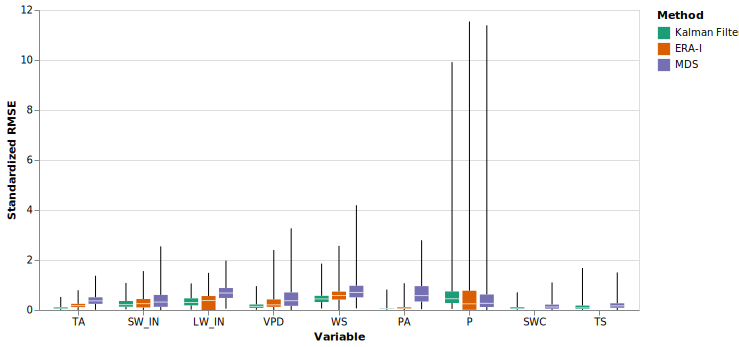
\includegraphics[width=\imgwidth]{the_plot_stand}}
\caption{Box plot to compare Standardized Root Mean Square Error(RMSE) for each variable between the different methods: Kalman Filter and the state of the art methods ERA and MDS. The same data from figure \ref{fig:the_plot} has been aggregated for all gap lengths}
\label{fig:the_plot_stand}
\end{figure}


\begin{table}
\centering
\caption{Comparison of imputation methods using Standardized RMSE. The best method for each gap length is highligthed in bold}
\label{the_table_stand}
\begin{tabular}{p{2.1cm}c|rr|rr|rr}
\toprule
 &  & \multicolumn{2}{r}{KalmanFilter} & \multicolumn{2}{r}{ERA} & \multicolumn{2}{r}{MDS} \\
 & RMSE & mean & std & mean & std & mean & std \\
Variable & Gap [$h$] &  &  &  &  &  &  \\
\midrule
\multirow[c]{4}{*}{\parbox{2.1cm}{\textbf{TA}}} & 6 & \bfseries 0.063 & 0.037 & 0.171 & 0.129 & 0.337 & 0.239 \\
 & 12 & \bfseries 0.087 & 0.052 & 0.176 & 0.110 & 0.367 & 0.209 \\
 & 24 & \bfseries 0.107 & 0.058 & 0.191 & 0.098 & 0.363 & 0.192 \\
 & 168 & \bfseries 0.137 & 0.055 & 0.223 & 0.077 & 0.468 & 0.153 \\
\cline{1-8}
\multirow[c]{4}{*}{\parbox{2.1cm}{\textbf{SW\_IN}}} & 6 & \bfseries 0.229 & 0.211 & 0.258 & 0.337 & 0.329 & 0.435 \\
 & 12 & \bfseries 0.252 & 0.173 & 0.279 & 0.248 & 0.372 & 0.367 \\
 & 24 & \bfseries 0.287 & 0.154 & 0.328 & 0.211 & 0.432 & 0.303 \\
 & 168 & \bfseries 0.299 & 0.121 & 0.337 & 0.168 & 0.519 & 0.258 \\
\cline{1-8}
\multirow[c]{4}{*}{\parbox{2.1cm}{\textbf{LW\_IN}}} & 6 & \bfseries 0.254 & 0.189 & 0.321 & 0.295 & 0.642 & 0.350 \\
 & 12 & \bfseries 0.321 & 0.201 & 0.362 & 0.295 & 0.695 & 0.335 \\
 & 24 & \bfseries 0.355 & 0.194 & 0.367 & 0.295 & 0.682 & 0.282 \\
 & 168 & 0.412 & 0.170 & \bfseries 0.399 & 0.266 & 0.776 & 0.219 \\
\cline{1-8}
\multirow[c]{4}{*}{\parbox{2.1cm}{\textbf{VPD}}} & 6 & \bfseries 0.136 & 0.100 & 0.304 & 0.360 & 0.489 & 0.507 \\
 & 12 & \bfseries 0.194 & 0.133 & 0.289 & 0.286 & 0.467 & 0.458 \\
 & 24 & \bfseries 0.216 & 0.130 & 0.296 & 0.248 & 0.469 & 0.424 \\
 & 168 & \bfseries 0.288 & 0.142 & 0.373 & 0.245 & 0.601 & 0.429 \\
\cline{1-8}
\multirow[c]{4}{*}{\parbox{2.1cm}{\textbf{WS}}} & 6 & \bfseries 0.358 & 0.185 & 0.564 & 0.344 & 0.696 & 0.438 \\
 & 12 & \bfseries 0.440 & 0.197 & 0.593 & 0.325 & 0.758 & 0.465 \\
 & 24 & \bfseries 0.504 & 0.242 & 0.615 & 0.297 & 0.795 & 0.465 \\
 & 168 & \bfseries 0.569 & 0.191 & 0.655 & 0.202 & 0.924 & 0.353 \\
\cline{1-8}
\multirow[c]{4}{*}{\parbox{2.1cm}{\textbf{PA}}} & 6 & \bfseries 0.058 & 0.077 & 0.095 & 0.114 & 0.605 & 0.477 \\
 & 12 & \bfseries 0.068 & 0.070 & 0.094 & 0.085 & 0.710 & 0.520 \\
 & 24 & \bfseries 0.066 & 0.029 & 0.089 & 0.049 & 0.663 & 0.478 \\
 & 168 & \bfseries 0.082 & 0.077 & 0.103 & 0.082 & 0.923 & 0.451 \\
\cline{1-8}
\multirow[c]{4}{*}{\parbox{2.1cm}{\textbf{P}}} & 6 & 0.419 & 0.872 & 0.435 & 1.046 & \bfseries 0.418 & 0.999 \\
 & 12 & 0.435 & 0.784 & 0.438 & 0.924 & \bfseries 0.418 & 0.847 \\
 & 24 & \bfseries 0.537 & 0.827 & 0.553 & 0.955 & 0.545 & 0.935 \\
 & 168 & \bfseries 0.701 & 0.632 & 0.793 & 0.711 & 0.766 & 0.704 \\
\cline{1-8}
\multirow[c]{4}{*}{\parbox{2.1cm}{\textbf{SWC}}} & 6 & \bfseries 0.057 & 0.043 & nan & nan & 0.143 & 0.164 \\
 & 12 & \bfseries 0.069 & 0.053 & nan & nan & 0.146 & 0.163 \\
 & 24 & \bfseries 0.082 & 0.060 & nan & nan & 0.146 & 0.131 \\
 & 168 & \bfseries 0.171 & 0.116 & nan & nan & 0.210 & 0.166 \\
\cline{1-8}
\multirow[c]{4}{*}{\parbox{2.1cm}{\textbf{TS}}} & 6 & \bfseries 0.070 & 0.057 & nan & nan & 0.184 & 0.177 \\
 & 12 & \bfseries 0.108 & 0.088 & nan & nan & 0.186 & 0.172 \\
 & 24 & \bfseries 0.159 & 0.155 & nan & nan & 0.192 & 0.155 \\
 & 168 & \bfseries 0.256 & 0.149 & nan & nan & 0.271 & 0.161 \\
\cline{1-8}
\bottomrule
\end{tabular}
\end{table}

\subsection{Additional Time series}

\begin{figure}
\centerline{\includegraphics[width=\imgwidth]{images2/timeseries_1_1}}
\caption{Timeseries 1}
\label{fig:ts_2-1}
\end{figure}

\begin{figure}
\centerline{\includegraphics[width=\imgwidth]{images2/timeseries_2_1}}
\caption{Timeseries 1}
\label{fig:ts_2-2}
\end{figure}

\begin{figure}
\centerline{\includegraphics[width=\imgwidth]{images2/timeseries_1_2}}
\caption{Timeseries 1}
\label{fig:ts_3-1}
\end{figure}

\begin{figure}
\centerline{\includegraphics[width=\imgwidth]{images2/timeseries_2_2}}
\caption{Timeseries 1}
\label{fig:ts_3-2}
\end{figure}
\subsection{Additional Tables}

\begin{table}
\centering
\caption{RMSE Comparison Kalman filter for different gap lengths}
\label{gap_len}
\begin{tabular}{p{2.1cm}l|cccccccc}
\toprule
 &  & 1 & 3 & 6 & 12 & 24 & 48 & 72 & 168 \\
Variable & RMSE &  &  &  &  &  &  &  &  \\
\midrule
\parbox{2.1cm}{\textbf{TA}} & mean & 0.194 & 0.287 & 0.440 & 0.628 & 0.826 & 0.904 & 0.939 & 0.986 \\
\cline{1-10}
\parbox{2.1cm}{\textbf{SW\_IN}} & mean & 27.869 & 37.737 & 44.486 & 50.090 & 57.306 & 58.099 & 58.938 & 59.045 \\
\cline{1-10}
\parbox{2.1cm}{\textbf{LW\_IN}} & mean & 5.628 & 7.948 & 11.455 & 13.292 & 15.916 & 17.051 & 16.284 & 17.491 \\
\cline{1-10}
\parbox{2.1cm}{\textbf{VPD}} & mean & 0.180 & 0.319 & 0.501 & 0.688 & 0.946 & 0.957 & 1.062 & 1.105 \\
\cline{1-10}
\parbox{2.1cm}{\textbf{WS}} & mean & 0.361 & 0.495 & 0.616 & 0.770 & 0.830 & 0.906 & 0.917 & 0.914 \\
\cline{1-10}
\parbox{2.1cm}{\textbf{PA}} & mean & 0.022 & 0.034 & 0.048 & 0.053 & 0.059 & 0.068 & 0.066 & 0.070 \\
\cline{1-10}
\parbox{2.1cm}{\textbf{P}} & mean & 0.092 & 0.165 & 0.116 & 0.200 & 0.186 & 0.208 & 0.215 & 0.238 \\
\cline{1-10}
\parbox{2.1cm}{\textbf{SWC}} & mean & 0.187 & 0.332 & 0.453 & 0.617 & 0.752 & 0.910 & 0.959 & 1.460 \\
\cline{1-10}
\parbox{2.1cm}{\textbf{TS}} & mean & 0.152 & 0.232 & 0.382 & 0.591 & 0.677 & 0.995 & 1.358 & 1.663 \\
\cline{1-10}
\bottomrule
\end{tabular}
\end{table}


\begin{table}
\centering
\begin{tabular}{p{2.1cm}c|rr|rr|r}
\toprule
 & Gap & \multicolumn{2}{r}{Only one var} & \multicolumn{2}{r}{All variables} &  \\
 & RMSE Standardized & mean & std & mean & std & diff. \\
Variable & Gap [$h$] &  &  &  &  &  \\
\midrule
\multirow[c]{4}{*}{\parbox{2.1cm}{\textbf{TA}}} & 3 & \bfseries 0.029 & 0.024 & 0.049 & 0.048 & 0.020 \\
 & 6 & \bfseries 0.040 & 0.028 & 0.078 & 0.052 & 0.039 \\
 & 12 & \bfseries 0.073 & 0.050 & 0.129 & 0.083 & 0.056 \\
 & 15 & \bfseries 0.079 & 0.057 & 0.138 & 0.092 & 0.059 \\
\cline{1-7}
\multirow[c]{4}{*}{\parbox{2.1cm}{\textbf{SW\_IN}}} & 3 & \bfseries 0.199 & 0.205 & 0.202 & 0.244 & 0.003 \\
 & 6 & \bfseries 0.222 & 0.171 & 0.228 & 0.215 & 0.006 \\
 & 12 & \bfseries 0.260 & 0.167 & 0.284 & 0.221 & 0.024 \\
 & 15 & \bfseries 0.277 & 0.166 & 0.307 & 0.217 & 0.030 \\
\cline{1-7}
\multirow[c]{4}{*}{\parbox{2.1cm}{\textbf{LW\_IN}}} & 3 & 0.194 & 0.169 & \bfseries 0.187 & 0.174 & -0.007 \\
 & 6 & \bfseries 0.276 & 0.216 & 0.288 & 0.234 & 0.012 \\
 & 12 & \bfseries 0.325 & 0.197 & 0.328 & 0.223 & 0.002 \\
 & 15 & \bfseries 0.337 & 0.188 & 0.345 & 0.212 & 0.008 \\
\cline{1-7}
\multirow[c]{4}{*}{\parbox{2.1cm}{\textbf{VPD}}} & 3 & \bfseries 0.070 & 0.070 & 0.105 & 0.105 & 0.035 \\
 & 6 & \bfseries 0.103 & 0.097 & 0.161 & 0.141 & 0.059 \\
 & 12 & \bfseries 0.155 & 0.116 & 0.233 & 0.193 & 0.078 \\
 & 15 & \bfseries 0.183 & 0.134 & 0.286 & 0.227 & 0.103 \\
\cline{1-7}
\multirow[c]{4}{*}{\parbox{2.1cm}{\textbf{WS}}} & 3 & \bfseries 0.297 & 0.179 & 0.301 & 0.181 & 0.004 \\
 & 6 & \bfseries 0.366 & 0.202 & 0.371 & 0.211 & 0.005 \\
 & 12 & \bfseries 0.460 & 0.242 & 0.468 & 0.248 & 0.009 \\
 & 15 & \bfseries 0.481 & 0.230 & 0.494 & 0.249 & 0.013 \\
\cline{1-7}
\multirow[c]{4}{*}{\parbox{2.1cm}{\textbf{PA}}} & 3 & \bfseries 0.024 & 0.016 & 0.029 & 0.020 & 0.005 \\
 & 6 & \bfseries 0.036 & 0.027 & 0.041 & 0.032 & 0.005 \\
 & 12 & \bfseries 0.057 & 0.074 & 0.064 & 0.091 & 0.007 \\
 & 15 & \bfseries 0.061 & 0.090 & 0.064 & 0.099 & 0.003 \\
\cline{1-7}
\multirow[c]{4}{*}{\parbox{2.1cm}{\textbf{P}}} & 3 & 0.290 & 0.450 & \bfseries 0.283 & 0.460 & -0.007 \\
 & 6 & \bfseries 0.386 & 0.524 & 0.396 & 0.592 & 0.010 \\
 & 12 & \bfseries 0.390 & 0.550 & 0.393 & 0.640 & 0.003 \\
 & 15 & \bfseries 0.442 & 0.675 & 0.449 & 0.767 & 0.008 \\
\cline{1-7}
\multirow[c]{4}{*}{\parbox{2.1cm}{\textbf{SWC}}} & 3 & \bfseries 0.013 & 0.032 & 0.013 & 0.033 & 0.000 \\
 & 6 & \bfseries 0.017 & 0.025 & 0.022 & 0.030 & 0.004 \\
 & 12 & \bfseries 0.026 & 0.034 & 0.032 & 0.036 & 0.006 \\
 & 15 & \bfseries 0.034 & 0.040 & 0.041 & 0.053 & 0.007 \\
\cline{1-7}
\multirow[c]{4}{*}{\parbox{2.1cm}{\textbf{TS}}} & 3 & \bfseries 0.024 & 0.023 & 0.031 & 0.036 & 0.007 \\
 & 6 & \bfseries 0.046 & 0.044 & 0.065 & 0.055 & 0.019 \\
 & 12 & \bfseries 0.083 & 0.088 & 0.106 & 0.112 & 0.023 \\
 & 15 & \bfseries 0.114 & 0.114 & 0.138 & 0.137 & 0.024 \\
\cline{1-7}
\bottomrule
\end{tabular}
\end{table}


\begin{table}
\centering
\caption{RMSE Comparison Kalman filter with and without control variable. The best result for each for each gap length is highligthed in bold}
\label{control}
\begin{tabular}{p{2.1cm}c|rr|rr|r}
\toprule
 & type & \multicolumn{2}{r}{Use Control} & \multicolumn{2}{r}{No Control} &  \\
 & RMSE Standardized & mean & std & mean & std & diff. \\
Variable & Gap [$h$] &  &  &  &  &  \\
\midrule
\multirow[c]{4}{*}{\parbox{2.1cm}{\textbf{TA} [\si{°C}]}} & 6 & 0.158 & 0.107 & \bfseries 0.118 & 0.066 & 0.040 \\
 & 12 & \bfseries 0.185 & 0.097 & 0.194 & 0.110 & 0.008 \\
 & 24 & \bfseries 0.254 & 0.133 & 0.274 & 0.164 & 0.021 \\
 & 168 & 0.267 & 0.065 & \bfseries 0.249 & 0.104 & 0.018 \\
\cline{1-7}
\multirow[c]{4}{*}{\parbox{2.1cm}{\textbf{SW\_IN} [\si{W/m^2}]}} & 6 & \bfseries 0.289 & 0.179 & 0.347 & 0.217 & 0.058 \\
 & 12 & \bfseries 0.345 & 0.177 & 0.524 & 0.285 & 0.179 \\
 & 24 & \bfseries 0.408 & 0.167 & 0.570 & 0.267 & 0.162 \\
 & 168 & \bfseries 0.435 & 0.124 & 0.597 & 0.232 & 0.161 \\
\cline{1-7}
\multirow[c]{4}{*}{\parbox{2.1cm}{\textbf{LW\_IN} [\si{W/m^2}]}} & 6 & 0.382 & 0.222 & \bfseries 0.300 & 0.179 & 0.082 \\
 & 12 & \bfseries 0.449 & 0.228 & 0.465 & 0.183 & 0.016 \\
 & 24 & \bfseries 0.487 & 0.190 & 0.534 & 0.185 & 0.047 \\
 & 168 & \bfseries 0.569 & 0.141 & 0.643 & 0.147 & 0.074 \\
\cline{1-7}
\multirow[c]{4}{*}{\parbox{2.1cm}{\textbf{VPD} [\si{hPa}]}} & 6 & 0.212 & 0.122 & \bfseries 0.202 & 0.198 & 0.009 \\
 & 12 & \bfseries 0.259 & 0.126 & 0.270 & 0.172 & 0.011 \\
 & 24 & \bfseries 0.373 & 0.184 & 0.383 & 0.332 & 0.009 \\
 & 168 & \bfseries 0.378 & 0.127 & 0.396 & 0.155 & 0.018 \\
\cline{1-7}
\multirow[c]{4}{*}{\parbox{2.1cm}{\textbf{WS} [\si{m/s}]}} & 6 & \bfseries 0.404 & 0.210 & 0.425 & 0.255 & 0.021 \\
 & 12 & \bfseries 0.544 & 0.194 & 0.616 & 0.290 & 0.071 \\
 & 24 & \bfseries 0.617 & 0.230 & 0.817 & 0.328 & 0.200 \\
 & 168 & \bfseries 0.695 & 0.208 & 0.900 & 0.293 & 0.206 \\
\cline{1-7}
\multirow[c]{4}{*}{\parbox{2.1cm}{\textbf{PA} [\si{hPa}]}} & 6 & \bfseries 0.123 & 0.090 & 0.146 & 0.087 & 0.024 \\
 & 12 & \bfseries 0.164 & 0.105 & 0.333 & 0.206 & 0.170 \\
 & 24 & \bfseries 0.179 & 0.065 & 0.655 & 0.387 & 0.476 \\
 & 168 & \bfseries 0.224 & 0.110 & 0.928 & 0.422 & 0.704 \\
\cline{1-7}
\multirow[c]{4}{*}{\parbox{2.1cm}{\textbf{P} [\si{mm}]}} & 6 & \bfseries 0.440 & 0.888 & 0.635 & 1.561 & 0.195 \\
 & 12 & 0.648 & 1.766 & \bfseries 0.543 & 0.627 & 0.105 \\
 & 24 & \bfseries 0.501 & 0.687 & 0.767 & 1.462 & 0.266 \\
 & 168 & \bfseries 0.793 & 0.707 & 0.822 & 0.751 & 0.029 \\
\cline{1-7}
\multirow[c]{4}{*}{\parbox{2.1cm}{\textbf{SWC} [\si{\%}]}} & 6 & 0.201 & 0.127 & \bfseries 0.122 & 0.090 & 0.078 \\
 & 12 & 0.345 & 0.206 & \bfseries 0.286 & 0.164 & 0.058 \\
 & 24 & 0.627 & 0.312 & \bfseries 0.495 & 0.252 & 0.131 \\
 & 168 & 0.812 & 0.390 & \bfseries 0.741 & 0.308 & 0.071 \\
\cline{1-7}
\multirow[c]{4}{*}{\parbox{2.1cm}{\textbf{TS} [\si{°C}]}} & 6 & 0.168 & 0.160 & \bfseries 0.132 & 0.090 & 0.035 \\
 & 12 & 0.230 & 0.139 & \bfseries 0.197 & 0.116 & 0.033 \\
 & 24 & 0.314 & 0.187 & \bfseries 0.264 & 0.197 & 0.051 \\
 & 168 & 0.358 & 0.136 & \bfseries 0.348 & 0.166 & 0.010 \\
\cline{1-7}
\bottomrule
\end{tabular}
\end{table}


\begin{table}
\centering
\begin{tabular}{p{2.1cm}c|rr|rr|r}
\toprule
 & type & \multicolumn{2}{r}{Generic} & \multicolumn{2}{r}{Finetuned one var} &  \\
 & RMSE Standardized & std & mean & std & mean & diff. \\
Variable & Gap [$h$] &  &  &  &  &  \\
\midrule
\multirow[c]{4}{*}{\parbox{2.1cm}{\textbf{TA} [\si{°C}]}} & 6 & 0.099 & 0.161 & \bfseries 0.046 & 0.065 & 0.096 \\
 & 12 & 0.112 & 0.210 & \bfseries 0.042 & 0.081 & 0.129 \\
 & 24 & 0.106 & 0.225 & \bfseries 0.061 & 0.112 & 0.113 \\
 & 168 & 0.099 & 0.274 & \bfseries 0.060 & 0.136 & 0.138 \\
\cline{1-7}
\multirow[c]{4}{*}{\parbox{2.1cm}{\textbf{SW\_IN} [\si{W/m^2}]}} & 6 & 0.234 & 0.302 & \bfseries 0.225 & 0.260 & 0.042 \\
 & 12 & 0.220 & 0.374 & \bfseries 0.200 & 0.275 & 0.099 \\
 & 24 & 0.185 & 0.420 & \bfseries 0.148 & 0.285 & 0.135 \\
 & 168 & 0.146 & 0.453 & \bfseries 0.115 & 0.294 & 0.158 \\
\cline{1-7}
\multirow[c]{4}{*}{\parbox{2.1cm}{\textbf{LW\_IN} [\si{W/m^2}]}} & 6 & \bfseries 0.216 & 0.376 & 0.219 & 0.330 & 0.046 \\
 & 12 & 0.331 & 0.477 & \bfseries 0.227 & 0.365 & 0.112 \\
 & 24 & \bfseries 0.196 & 0.531 & 0.200 & 0.370 & 0.161 \\
 & 168 & \bfseries 0.154 & 0.545 & 0.162 & 0.396 & 0.149 \\
\cline{1-7}
\multirow[c]{4}{*}{\parbox{2.1cm}{\textbf{VPD} [\si{hPa}]}} & 6 & 0.122 & 0.223 & \bfseries 0.072 & 0.126 & 0.096 \\
 & 12 & \bfseries 0.117 & 0.250 & 0.129 & 0.184 & 0.066 \\
 & 24 & \bfseries 0.132 & 0.327 & 0.156 & 0.269 & 0.058 \\
 & 168 & 0.151 & 0.391 & \bfseries 0.148 & 0.273 & 0.118 \\
\cline{1-7}
\multirow[c]{4}{*}{\parbox{2.1cm}{\textbf{WS} [\si{m/s}]}} & 6 & 0.272 & 0.417 & \bfseries 0.184 & 0.363 & 0.055 \\
 & 12 & 0.291 & 0.590 & \bfseries 0.189 & 0.409 & 0.180 \\
 & 24 & \bfseries 0.222 & 0.598 & 0.254 & 0.537 & 0.061 \\
 & 168 & 0.243 & 0.778 & \bfseries 0.197 & 0.573 & 0.206 \\
\cline{1-7}
\multirow[c]{4}{*}{\parbox{2.1cm}{\textbf{PA} [\si{hPa}]}} & 6 & 0.077 & 0.110 & \bfseries 0.031 & 0.049 & 0.061 \\
 & 12 & 0.089 & 0.164 & \bfseries 0.031 & 0.065 & 0.099 \\
 & 24 & 0.090 & 0.195 & \bfseries 0.035 & 0.070 & 0.125 \\
 & 168 & 0.085 & 0.219 & \bfseries 0.045 & 0.078 & 0.142 \\
\cline{1-7}
\multirow[c]{4}{*}{\parbox{2.1cm}{\textbf{P} [\si{mm}]}} & 6 & \bfseries 0.634 & 0.325 & 0.636 & 0.371 & 0.045 \\
 & 12 & 0.873 & 0.563 & \bfseries 0.769 & 0.482 & 0.081 \\
 & 24 & 0.906 & 0.531 & \bfseries 0.678 & 0.522 & 0.009 \\
 & 168 & 0.731 & 0.735 & \bfseries 0.502 & 0.633 & 0.102 \\
\cline{1-7}
\multirow[c]{4}{*}{\parbox{2.1cm}{\textbf{SWC} [\si{\%}]}} & 6 & 0.126 & 0.212 & \bfseries 0.038 & 0.055 & 0.157 \\
 & 12 & 0.200 & 0.337 & \bfseries 0.037 & 0.063 & 0.274 \\
 & 24 & 0.290 & 0.586 & \bfseries 0.070 & 0.090 & 0.495 \\
 & 168 & 0.345 & 0.782 & \bfseries 0.104 & 0.180 & 0.601 \\
\cline{1-7}
\multirow[c]{4}{*}{\parbox{2.1cm}{\textbf{TS} [\si{°C}]}} & 6 & 0.117 & 0.156 & \bfseries 0.065 & 0.076 & 0.081 \\
 & 12 & 0.130 & 0.238 & \bfseries 0.078 & 0.100 & 0.139 \\
 & 24 & 0.176 & 0.292 & \bfseries 0.106 & 0.150 & 0.142 \\
 & 168 & 0.174 & 0.377 & \bfseries 0.154 & 0.257 & 0.120 \\
\cline{1-7}
\bottomrule
\end{tabular}
\end{table}


\begin{table}
\centering
\caption{\CapTrain}
\label{tbl:train_compare}
\begin{tabular}{p{2.1cm}l|rr|rr|rr}
\toprule
 & Train & \multicolumn{2}{r}{Multi vars} & \multicolumn{2}{r}{Only one var} & \multicolumn{2}{r}{Random params} \\
 & Stand. RMSE & mean & std & mean & std & mean & std \\
Variable & Gap [$h$] &  &  &  &  &  &  \\
\midrule
\multirow[c]{4}{*}{\textbf{TA}} & 3 h & \bfseries 0.029 & 0.024 & 0.066 & 0.050 & 0.060 & 0.045 \\
 & 6 h & \bfseries 0.044 & 0.033 & 0.093 & 0.062 & 0.080 & 0.055 \\
 & 12 h & \bfseries 0.073 & 0.050 & 0.133 & 0.092 & 0.117 & 0.085 \\
 & 15 h & \bfseries 0.077 & 0.051 & 0.131 & 0.072 & 0.111 & 0.068 \\
\cline{1-8}
\multirow[c]{4}{*}{\textbf{SW\_IN}} & 3 h & \bfseries 0.178 & 0.176 & 0.202 & 0.178 & 0.259 & 0.220 \\
 & 6 h & \bfseries 0.210 & 0.170 & 0.249 & 0.176 & 0.283 & 0.209 \\
 & 12 h & \bfseries 0.269 & 0.172 & 0.308 & 0.167 & 0.333 & 0.193 \\
 & 15 h & \bfseries 0.270 & 0.166 & 0.315 & 0.164 & 0.334 & 0.188 \\
\cline{1-8}
\multirow[c]{4}{*}{\textbf{LW\_IN}} & 3 h & \bfseries 0.200 & 0.169 & 0.215 & 0.177 & 0.298 & 0.203 \\
 & 6 h & \bfseries 0.270 & 0.216 & 0.297 & 0.229 & 0.342 & 0.229 \\
 & 12 h & \bfseries 0.332 & 0.224 & 0.377 & 0.241 & 0.398 & 0.259 \\
 & 15 h & \bfseries 0.357 & 0.208 & 0.390 & 0.208 & 0.398 & 0.225 \\
\cline{1-8}
\multirow[c]{4}{*}{\textbf{VPD}} & 3 h & \bfseries 0.064 & 0.060 & 0.097 & 0.079 & 0.150 & 0.128 \\
 & 6 h & \bfseries 0.098 & 0.096 & 0.148 & 0.113 & 0.193 & 0.174 \\
 & 12 h & \bfseries 0.168 & 0.156 & 0.223 & 0.161 & 0.240 & 0.192 \\
 & 15 h & \bfseries 0.186 & 0.159 & 0.241 & 0.168 & 0.254 & 0.210 \\
\cline{1-8}
\multirow[c]{4}{*}{\textbf{WS}} & 3 h & \bfseries 0.305 & 0.183 & 0.471 & 0.460 & 0.447 & 0.300 \\
 & 6 h & \bfseries 0.372 & 0.210 & 0.576 & 0.466 & 0.482 & 0.309 \\
 & 12 h & \bfseries 0.429 & 0.195 & 0.649 & 0.481 & 0.523 & 0.270 \\
 & 15 h & \bfseries 0.479 & 0.230 & 0.691 & 0.457 & 0.540 & 0.293 \\
\cline{1-8}
\multirow[c]{4}{*}{\textbf{PA}} & 3 h & \bfseries 0.025 & 0.019 & 0.073 & 0.062 & 0.067 & 0.057 \\
 & 6 h & \bfseries 0.035 & 0.021 & 0.095 & 0.061 & 0.098 & 0.077 \\
 & 12 h & \bfseries 0.051 & 0.045 & 0.117 & 0.073 & 0.118 & 0.089 \\
 & 15 h & \bfseries 0.059 & 0.040 & 0.128 & 0.080 & 0.115 & 0.076 \\
\cline{1-8}
\multirow[c]{4}{*}{\textbf{P}} & 3 h & \bfseries 0.348 & 0.680 & 0.411 & 1.510 & 0.371 & 0.713 \\
 & 6 h & \bfseries 0.400 & 0.618 & 0.487 & 0.718 & 0.425 & 0.704 \\
 & 12 h & \bfseries 0.511 & 0.851 & 0.706 & 1.150 & 0.535 & 0.981 \\
 & 15 h & \bfseries 0.453 & 0.598 & 0.618 & 0.756 & 0.470 & 0.698 \\
\cline{1-8}
\multirow[c]{4}{*}{\textbf{SWC}} & 3 h & \bfseries 0.012 & 0.029 & 0.095 & 0.076 & 0.106 & 0.075 \\
 & 6 h & \bfseries 0.018 & 0.031 & 0.151 & 0.108 & 0.153 & 0.107 \\
 & 12 h & \bfseries 0.027 & 0.037 & 0.245 & 0.160 & 0.246 & 0.215 \\
 & 15 h & \bfseries 0.033 & 0.041 & 0.282 & 0.228 & 0.278 & 0.208 \\
\cline{1-8}
\multirow[c]{4}{*}{\textbf{TS}} & 3 h & \bfseries 0.024 & 0.018 & 0.102 & 0.082 & 0.047 & 0.037 \\
 & 6 h & \bfseries 0.048 & 0.048 & 0.164 & 0.106 & 0.076 & 0.074 \\
 & 12 h & \bfseries 0.083 & 0.086 & 0.231 & 0.158 & 0.122 & 0.134 \\
 & 15 h & \bfseries 0.117 & 0.129 & 0.271 & 0.191 & 0.154 & 0.161 \\
\cline{1-8}
\bottomrule
\end{tabular}
\end{table}



\subsection{Gap length distribution in FLUXNET}



The entire FLUXNET 2015 dataset was used to compute the distribution of gap lengths across the all the sites for each variable. A gap was definite when the QC flag of the variable is different from 0 or the data itself is missing. Figure \ref{fig:gap_len_dist} shows the complete distribution of the gaps, while figure \ref{fig:gap_len_dist_small} focuses only on gaps shorter than a week.


\begin{figure}
\centerline{\includegraphics[width=\imgwidth]{gap_len_dist}}
\caption{FLUXNET gap len}
\label{fig:gap_len_dist}
\end{figure}
\begin{figure}
\centerline{\includegraphics[width=\imgwidth]{gap_len_dist_small}}
\caption{FLUXNET gap len less than a week}
\label{fig:gap_len_dist_small}
\end{figure}



\section{Comparison between Standard and Square Root Kalman Filter}

\begin{figure}
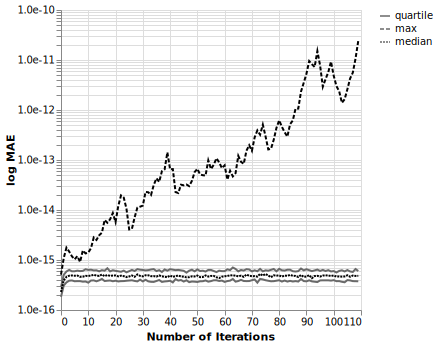
\includegraphics[width=\textwidth]{numerical_stability}
 \caption{\textbf{Numerical stability} comparison between standard Kalman Filter implementation and Square Root Filter. For 100 times the filter has been initialized with random parameters (drawn from a uniform distribution range 0-1) and then filtered 100 observations. At each filter iteration the Mean Absolute Error (MAE) was calculated between the state covariance from the standard filter and the square root filter. The plot shows the median, 1 and 3 quartile and the maximum of the MAE across the 100 samples.}
\end{figure}

\begin{figure}
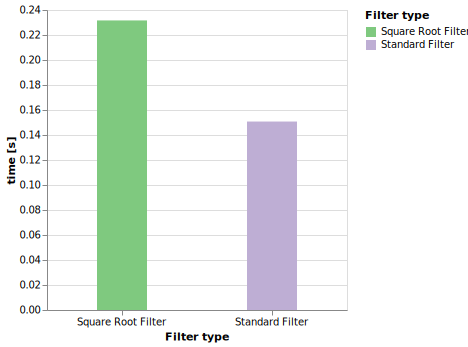
\includegraphics[width=\textwidth]{perf_sr}
 \caption{\textbf{Performance} comparison between standard Kalman Filter implementation and Square Root Filter. 100 samples with the following settings: Number of observations: 100, dimension observations 4, dimension state: 3, dimension control: 3, batch size: 5. Data and parameters are randomly generated.}
\end{figure}


% \section{Detailed Notation}

% \begin{itemize}
% \item $t$  Number of time steps
% \item observations
% \begin{itemize}
%     \item $n$  Number of variables observed
%     \item $y_{:,t}$ or $y_t$ vector of all the $n$ variables at time $t$, $\in \mathbb{R}^n $
%     \item $y_{n,:}$ vector of the $n$th variable at for time steps in $t$, $\in \mathbb{R}^T$
%     \item $y_{n,t}$ $n$th variable at time $t$, $\in \mathbb{R}$ 
%     \item $Y_M = [x_{:,1}, ... x_{:, t}]$ Matrix with all the $n$ variables at all time steps, $\in \mathbb{R}^{n \times t}$ 
%     \item $Y$ is a vector obtained by "flattening" $X_M$, by putting next to each other all variable at time $t$, $\in \mathbb{R}^{(n \cdot t)}$
%     \item $y^{ng}_t$ vector of variable that are not missing (ng = not gap)) at time $t$, $\in \mathbb{R}^{n_{ng}}$. Note at different times the shape of this vector can change
%     \item $Y^{ng}$ all observations
% \end{itemize}

% \item Latent state
% \begin{itemize}
%     \item $k$  Number of variables in latent state
%     \item $x_{:,t}$ or $x_t$ vector of all the $k$ state variables at time $t$, $\in \mathbb{R}^k $
%     \item $x_{k,:}$ vector of the $k$th variable at for time steps in $t$, $\in \mathbb{R}^t$
%     \item $x_{k,t}$ $k$th variable at time $t$, $\in \mathbb{R}$ 
%     \item $X_M = [x_{:,1}, ... x_{:, t}]$ Matrix with all the $k$ variables at all time steps, $\in \mathbb{R}^{k \times t}$ 
%     \item $X$ is a vector obtained by "flattening" $X_M$, by putting next to each other all variable at time $t$, $\in \mathbb{R}^{(k \cdot t)}$
% \end{itemize}

% \end{itemize}

\end{document}

